
%
% sample.tex
% $Id: sample.tex,v 1.1 2006/03/18 00:21:36 johnh Exp johnh $
%


% The default of sigplan-proc-varsize is 9pt, indented paragraphs (acm style)
% For Sensys or other 10pt conference, use the 10pt option
%\documentclass{sigplan-proc-varsize}
% options:
%\documentclass[9pt]{sigplan-proc-varsize}
\documentclass[10pt]{sigplan-proc-varsize}
%\documentclass[noindentedparagraphs]{sigplan-proc-varsize}



% % hack to avoid the ugly ACM paragraph definition
% % => can't leave blank line after this
% (remove comment for this hack)
% \renewcommand{\paragraph}[1]{\vskip 6pt\noindent\textbf{#1 }}
\usepackage{amsmath}
\usepackage{graphicx}
\usepackage{url}
\usepackage{underscore}


\numberofauthors{1}


\author{
%
% The command \alignauthor (no curly braces needed) should
% precede each author name, affiliation/snail-mail address and
% e-mail address. Additionally, tag each line of
% affiliation/address with \affaddr, and tag the
%% e-mail address with \email.
\alignauthor Vijay Akkineni \\
        \affaddr{Department of Computer Science and Engineering}\\
        \affaddr{Georgia State University}\\
       \email{vakkineni1@student.gsu.edu}
}

\title{Fault localization in Communication Networks}

%\conferenceinfo{Phd Qualifiers'13,} {September 6, 2013, Atlanta, United States.}
%\CopyrightYear{2013}

\begin{document}

\maketitle

\begin{abstract}
This paper is about fault localization techniques in communication networks worked for Phd qualifiers examination. 
Fault Localization is an important aspect of network fault management and is a process of deducing the source of a failure from the set of observed indicatations. 
It has been an important research area in the field of networking both communication networks and wireless sensor networks.
As commuication networks grow in size and complexity it has been imposing new set of requirements on fault localization. 
Despite the amount of research done in this field we can still argue that it is an area of open for research. 
The paper essentially disucsses the work that has been done in this field in the pas few years with emphasis on the both the papers given for the examination.
\end{abstract}

% A category with the (minimum) three required fields
\category{H.4}{Communication Networks, Sensor Network Applications}{Miscellaneous}

\keywords{Fault Localization, Communication Networks, Root Cause Analysis, Causal Inference}

\section{Introduction}
  \label{sec:intro}

Fault diagnosis is an important part of networking. Faults are unavoidable in communication systems but their quick detection and isolation and repair is critical 
for the robustness, reliability and health of the system. When the networks get large and cumbersome automatic fault diagnosis and fault management is a crucial aspect.

A basic taxonomy in this field is mentioned below.

Event, defined as an exceptional condition occurring in the operation of hardware or software of a managed network, is a central concept pertaining to fault diagnosis.

Faults (also referred to as problems or root causes) constitute a class of network events that can cause other events but are not themselves caused by other 
events. Faults may be classified as: (1) permanent, (2) intermittent, and (3) transient. A permanent fault exists in a network until a repair action is taken.
Intermittent faults occur on a discontinuous and periodic basis causing a degradation of service for short periods of time.
However, frequently re-occurring intermittent faults significantly jeopardize service performance. 
Transient faults cause a temporary and minor degradation of service.

Error(Failure) is defined as a discrepancy between a computed, observed, or measured value or condition and a true, specified, or theoretically correct value or condition. 
Error is a consequence of a fault. Faults may or may not cause one or more errors. 
Errors may cause deviation of a delivered service from the specified service, which is visible to the outside world. 
Errors do not need to be directly corrected, and in many cases they are not visible externally. 
However, an error in a network device or software may cause a malfunctioning of dependent network devices or software. 
Thus, errors may propagate within the network causing failures of faultless hardware or software.

Symptoms are external manifestations of failures. They are observed as alarms—notifications of a potential failure. 
These notifications may originate from management agents via management protocol messages (SNMP trap and CMIP EVENT-REPORT), 
from management systems that monitor the network status, e.g., using command ping, system log-files or character streams sent by external equipments.

Figure 1 shows the concepts described above in an end to end perspective.

The process of fault diagnosis usually involves three steps as cited in \cite{KatzelaThesis:1996}:

\begin{itemize}
  \item Fault detection, a process of capturing on-line indications of network disorder provided by malfunctioning devices or fault detection agents in the 
  form of alarms.
  \item Fault localization (also referred to as fault isolation, alarm/event correlation, and root cause analysis) is a set of observed fault indications is analyzed to 
  find an explanation of the alarms.
  \item Testing is a process that, given a number of possible explanations, determines the actual faults.
  \item Fault Correction, by which we mean not only to diagnose, but
also to repair all faulty components within a network (This includes the testing component).
\end{itemize}

\begin{figure}[h!]
  \caption{Distinction between fault, error and symptom}
  \centering
    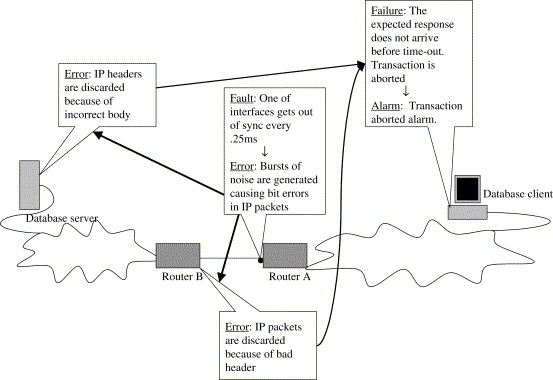
\includegraphics[width=0.5\textwidth]{Fig1}
\end{figure}

The difficulty in the fault localization process arise from the ambiguity of the observed set of alarms as same alarm can be generated from multiple different faults 
and multiple alarms can correlate back to the same fault. The incompleteness of the alarm stems from the fact that the alarm doesn't have all the information or 
there is a loss of alarm. Inconsistency among the observed alarms results from device perception of the fault is different form device to device.  

A set of alarms generated by a fault may depend on many factors such as dependencies among network devices, current configurations, services in use since 
fault occurrence, presence of other faults, values of other network parameters, etc. Due to this non-determinism the system knowledge may be subject to inaccuracy 
and inconsistency. Fault evidence may also be inaccurate because of spurious alarms, which are generated by transient problems or as a result of overly sensitive 
fault detection mechanisms. When spurious symptoms may occur, the management system may not be sure which observed alarms should be taken into account in the fault 
localization process. Event management systems should identify and eliminate multiple simultaneous related or unrelated root causes. 

In large networks distributed fault localization process should be performed in distributed fashion. Many researches \cite{Katzela:1995} and \cite{Yemini:1996} have 
concluded that distributed fault localization using a set of event management nodes is a better approach than centralized process. The complexity arised from the nature 
of error propogation, they propogate either horizontally to the peers or vertically from bottom layer to upper layers or afecting higher level services. The errors also
propogate from one management domain to a different management domain making the process even difficult. Therefore the distribution of complexity to distributed fault 
localization processes and inferring form the collective process makes the process computationally feasible and efficient. 

An alarm can insinuate different type of faults that occurred in different communication devices where in fault localization process may not comeup with a 
definitive answer. Few approaches that will be discussed in this paper combine fault localization with testing and fault ocrrection process to validate the hypothesis. 
Therefore there should be some kind of optimality measure or confidence measure that should be employed in measuring the hypothesis that the localization process 
came up with and it could include the lowest cost or min failure probability or some heuristic function which optimizes the process of validating the hypothesis.

Numerous works have been proposed on fault localization process. The techniques are dervice from different areas of artificial intelligence, graph theory, 
neural networks, automata theory and many other approaches. Figure 2 broadly classifies the exisiting solutions. The two papers provided for the exam falls into the 
category of end to end testing scenarios and proababilistic reasoning and derive their roots from bayesian network analysis. 

\begin{figure}[h!]
  \caption{Classification of fault localization techniques}
  \centering
    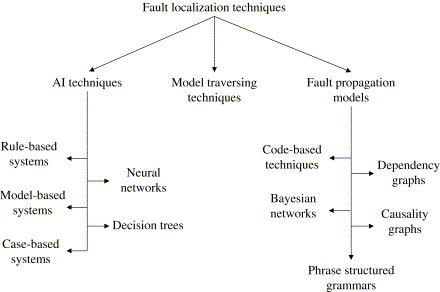
\includegraphics[width=0.5\textwidth]{Fig2}
\end{figure}

This paper presents the background research that has been done before paper 1 in section 2 - 4 and in section 5 presents the paper 1 \cite{pclee:07}.

\section{Expert Systems techniques}
Most widely used technique in the field of fault localization and diagnosis are expert systems as they try to mimic the actions of human expert. 
Most expert systems use rule based system as their inference engine. \cite{Peng:97},\cite{Liu:99} and \cite{Nygate:95} are examples of expert systems.

The expert systems developed differ in the knowledge they use. Rule based fault localization solely depend on the 
structure of the knowledge base as rule definition language. In \cite{Lor:93}   the knowledge base is divided to reusable 
knowledge modeled as core knowledge and customized knowledge.  in  \cite{Liu:99} the rules are organized as composite events and 
an intervention of human expert is required to update the event base.  The rule based systems can act as a powerful tool to eliminate 
least likely hypothesis. Although the RBR paradigm is appropriate for problem-solving tasks that are confined and well-understood its limitations are.

\begin{itemize}
  \item an in-ability to learn from experience.
  \item Fan inability to deal with novel problems.
  \item the difxulty of updating the systems to keep up with rapidiy changing domains such as expanding heterogeneous network.
\end{itemize}

in Model bases expert systems like \cite{Nygate:95} conditions are ususally accosiated with rules which includes predicates referring to system model. 
These predicates test the syetem for existence of relationship among system component. \cite{Nygate:95} 
uses correlation tree skeletons describing cause and effect relation ships between event. regardless of what expert system is being used localization process is 
always driven by inference engine and correaltion rules between events. 

\cite{Lewis:93} and \cite{Gardner:96} are examples of Case-based reasoning systems. The goals of CBR systems are (i) to learn from experience, (ii) to 
offer solutions to novel problems based on past experience, and (iii) to avoid expensive maintenance. The basic idea of CBR is to recall, adapt, and 
execute episodes of former problem-solving in an attempt to deal with a current problem. Former episodes of problem-solving are represented as cases in a case 
library. When confronted with a new problem, a CBR system retrieves a similar case and tries to adapt the case in an attempt to solve the outstanding problem. 
The disadvantages of such a system is the time complexity in retrieving a case that is the closest match to the event and the close tailoring of the application 
to the domain.

In addition to the above mentioned techniques there are other notable techniques are neural networks based approaches \cite{Gardner:97} \cite{Gardner:98} and 
decision tree based approaches \cite{Rodosek:98}. Neural networks have parallel computing architecture and are very fast avoiding bottlenecks which 
commonly arises from serial processing. But the main disadvantage is that the learning process requires intesive training  and in communication networks 
where all the alarms signatures are not readily available for pattern recognition.

Decision tree aproaches are simple and allows expressive representation of expert knowledge howeever they are limited by the dependencies sepcific 
applications nad degraded accuracy in noisy scenarios \cite{Russell:96} \cite{Koller:10}.

\section{Model traversing techniques}
\cite{Katker:96}, \cite{Katker:971}, \cite{Katker:97} and \cite{Gruschke:98} are all Model Traversing that use formal representation of communication 
system with clearly marked relationships across network entities. This technique identifies faults by traversing a model of entities starting form the entity whic reported an alarm and also involves a fault identification process to identify and locate faulty network entities.

The model representation used by this technique is object-oriented representation of the given system. It is based on the OSI management framework and uses GDMO (Guidelines for  Definition  of Managed Objects) with extensions to the MO to model dependencies and services between the entities. This approach can make automated testing possible which can test for various testing entities availability and quality of service standards. 

The event correlation in model traversing techniques is event driven as when an event occurs it is being mapped to the reported entity and the managed object representing that entity. For every event the search begins from the MO reporting the event and is searched recursively forllowing all relationship links between MO's using fault localization algorithms.  Fault localization algorithms used in this technique can be of various flavours.  models every event as singleton classes and merges them whenever they are traced to the same node. Typical proerties of such techniques involve 

\begin{itemize}
  \item Level at which a particular fault has occurred in the model.
  \item Event Type.
  \item Event severity.
  \item Event Origin - to identify if the event occurred is primary or secondary.
\end{itemize}

\begin{figure}[h!]
  \caption{Architecture of a model traversing technique prototype}
  \centering
    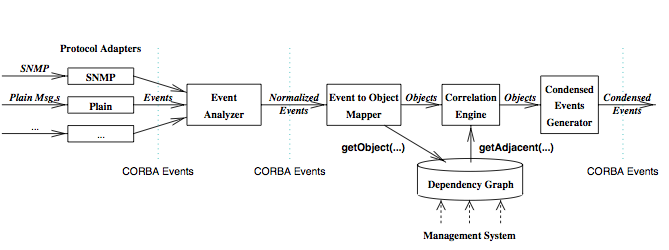
\includegraphics[width=0.5\textwidth]{Fig3}
\end{figure}

The MO's provide functions which lets the process test the entity for its operational status.  The root cause is found when the process stops at an entity and validates that it is a malfucntioning object and doesn't depend on any other object. In a multi layer model vertical search is performed first and then horizontal search in the next lower layer to check its peer at the end of search process votes are collected to identify the faulty elements and the device that recieves the most votes is declared faulty and a testing process kicks in to test the validity of the hypothesis. 

Model traversing techniques are pretty robust agianst network configuration changes and very useful in the scenario's where automated testing is a requirement and the depedency model is very natural as they are modeled as Trees or Graphs. 

The biggest drawback is the Fault Propagation Patterns and when there  fault is a logical combination of multiple devices and byzatine problems. It also incurs heavy testing costs. 

\section{Graph-theoretic techniques}
 
Grap theoretic techniques depend on gaphical model of a system called fault proppagation model(FPM). FPM represents fault and symptoms that occur in a system. 
The symptoms that are observed are mapped into nodes in the FPM and localization algorithms analyze the graph to infer the best explanation of the observed symptoms. 

These techniques require a knowlede of depedencies among the abstract and physical system components and how these failures in one component are related to 
other components. The success of the fault localiztion algorithm depends on the the accuracy of this a priori specification.

FPM's are genrally modeled as (i) Cuasaultiy graph is is a DAG whose nodes are events and edges represent the causality implications i.e cause effect relationships 
between events. They are carry probabilties to the nodes and edges implying the probability of a certain event to happen. 
Dependency Graph is a directed graph {\it{G=(O,D)}} where O represent a finite set of nodes and D are the depedency edges between Objects. 
The directed edge (o$_{i}$,o$_{j}$) $\in$ D represents that when o$_{i}$ fails o$_{j}$ fails or emits some kind of error. 
The edges are also labeled with conditional probabilities. Figure 4 represents such a depedency graph.

\begin{figure}[h!]
  \caption{A Network example along with the dependecy graph \cite{Katzela:95}}
  \centering
    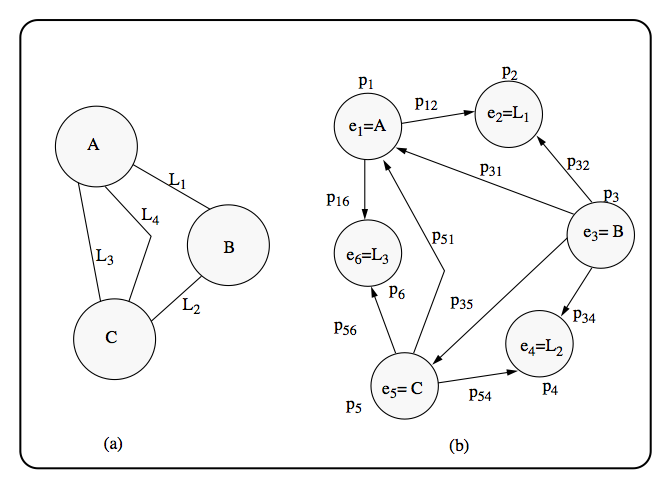
\includegraphics[width=0.5\textwidth]{Fig4}
\end{figure}

A lot of approaches using dependency graph, a critical assumption involves that an entity may fail in only one way. If that is the case the causal graph and dependecy graph would be the same.  In the case of multiple failures associated to a single entity they can be divided into sets such as {\it{complete failure, abnormal transmission delay, high packet loss, etc.}}. The dependecy graph in this case would have multiple edges between failure modes and the Object(entity). Sethi et all in \cite{Sethi:02}, \cite{Sethi:041}, \cite{Sethi:04} have modeled using multiple failure modes principle. 

A fault localalization algorithm, based on the provided FPM generally returns a number of hypothesis that best explain the observed symptoms. The problem of finding best explanation of the recieved alarms is {\it{NP-hard}} problem and proved in \cite{Katzela:95} by reducing the given problem to a Min Set-Cover problem.

\subsection{Divide and conquer algorithm}
The divide and conquer algorith uses a FPM assuming that one type of failure is allowed per object. It is a window based technique i.e gathers all the faults in a time window and analyzes them. 

System model is a directed graph G = ( E ,D) called the dependencygraph, where E is a finite nonempty set of active terminal objects e$_i$, and a directed edge (e$_i$, e$_j$) $\in$ D denotes the fact that a fault in e$_i$ has a side effect on e$_j$ i.e., e$_j$ is dependent on e$_i$.
Each vertex e$_i$ is assigned a weight p$_i$ that is the probability that the object e$_i$ fails independently of the state (failed or not failed) of any other active terminal object that is dependent on it. Each directed edge ( e$_j$,e$_i$) is assigned a weight p$_{ji}$ which represents the strength of dependency between the entities it connects. Specifically, p$_{ji}$ , is the conditional probability p$_{ji}$ = P(e$_j$ fails\textbar e$_i$ fails) that entity e$_j$, fails as a result of the failure of entity e$_i$. In addition, the weight of a directed path is defined as the product of all the weights of the edges that compose the path. Finally, the strength of dependency p$_{kl}$ between two non-adjacent vertices e$_k$ and e$_l$, is defined as the maximum of the weights of all directed paths from e$_k$ to e$_l$.

Let D(a$_i$) for every a$_i$ alarm be the domain of alarms that defines as the set of objects that might have caused the alarm.  The domain of an alarm calculation is a variation of single source problem that finds the min cost paths from a source vertex to all other graphs and the nodes are chosen such that the cost of path e$_i$ to e$_j$ is subject to restriction that we include only the minimum cost paths with cost $\leq$ log(W) where W is a parameter.

The outline of the algorithm run has been given below.

\begin{itemize}
  \item Start with the set S of objects associated with the alarm cluster.
  \item Find the partitioning of the set S resulting in two disjoint sets so in each set the objects exhibit the maximum mutual dependency, i.e., for every object e$_i$ and e$_j$, that belongs to the same set and e$_k$ that does not belong to the set, the dependency weight p$_{ij}$is greater than the dependency weights p$_{ik}$, p$_{ki}$, p$_{jk}$, p$_{kj}$.
  \item Of the two sets, select the one that explains all the received alarms and has the maximum probability that at least one of the entities in the set is a fault. If there is no such set then find the subset of alarms that each set explains and select both.
  \item Apply the previous two steps of the algorithm recursively to the selected sets until the resulting sets of the current partitioning are singletons.
\end{itemize}

By partitioning with the maximum mutual dependency criterion we group together objects that are highly dependent on each other and when the result of partitionining, both the sets are capable of explaingin all the alarms then we select one set that has higher probability of having one of them at fault. 

When determining atleast on memeber of the subset is faulty it is calcualted using. 

P(S) = ${\underset{\forall i:e_i \in S}{\sum}}[p_i + \underset{\forall j:e_j \in S , j \neq i}{\sum} p_{ij}.p_j]$


\begin{figure}[h!]
  \caption{Divide and Conquer algorithm \cite{Katzela:95}}
  \centering
    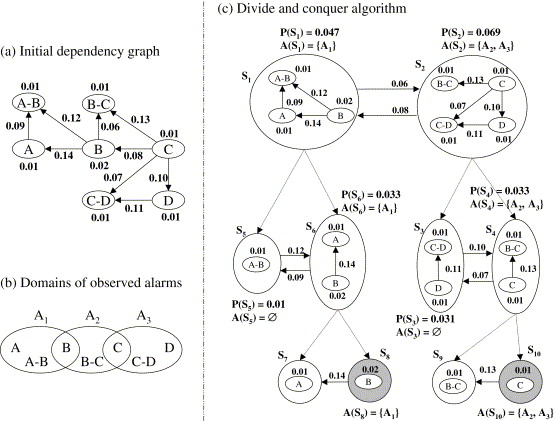
\includegraphics[width=0.5\textwidth]{Fig5}
\end{figure}

In algorithm runs in two phases where in the first phase algorithm finds the maximum mutual partitionings of the entities in the set S. The result of Phase I is a hierarchical clustering of the entities in the set S. In the Phase II a fault localization algorithm is recursively invoked to find the subsets that are supposed to be used. The first subcluster contains all alarms that may be explained using the subset with the higher probability that one of its members was a primary source of a failure. The second subcluster contains the remaining alarms from the original alarm cluster. Its domain is the other of the two subsets. The recursive procedure is then invoked twice, taking the two subclusters and their respective domains as parameters. The recursion continues until the input alarm cluster domain is a singleton. 

The algorithm mentioned above gives the explanation of the observed alarms but may not prouce the best output as it is a approximation algorithm based on maximum mutual dependency heuristic. The runtime complexity of the algorithm is O(N$^{3}$) and the partitioning phase runtime is O(logN). The drawback of the algorithm is it cannot handle the lost or spurious alarms and is a time window based determinsitic algorithm.

\subsection{Bayesian Reasoning approach}
Bayesian network or probabilistic graphical model represents a set of random varaibles and their conditional dependencies using a directed acyclic graph. In the context of fault localization the random variables represent the state of network entities and the occurrence of network events. 

\begin{figure}[h!]
  \caption{A example bayesian network}
  \centering
    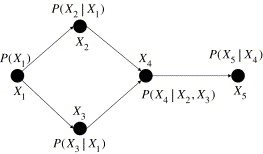
\includegraphics[width=0.5\textwidth]{Fig6}
\end{figure}

Belief networks are used to make four basic queries given evidence set e: belief assessment, most probable explanation, maximum a posteriori hypothesis, and maximum expected utililty \cite{Pearl:98}

\cite{Cynthia:97}, \cite{Sethi:02}, \cite{Sethi:041} and \cite{Sethi:04} all the papers try to model the FPM as a bayesian network using a layered fault model apparoach and in general fault component models are divided into services, protocols and functions. The recursive dependencies between services, protocols and functions constitue a dependenct graph. Uncertainty about dependencies between communication system entities is represented by assigning probabilities to the links and/or nodes in the dependency or causality graph. 

The queries for belief assesment and most probable explanation are of particular interest in the approaches mentioned above. The belief assesment task is to compute $bel(V_i=v_i) = P(V_i=v_i|e)$. given an evidence e, {\it bel}  gives the certainity of an event happening under the evidence. The most probable explanation task is to find an assignment that best explains the observed evidence e, i.e.,  \\
$P(A_{max}) = max_A \underset{i=1}{\overset{n}{\pi}} P(V_i=v_i^A | Par(V_i)^A)$ \cite{Pearl:98}. \\
It is known that the above tasks are NP-{\it hard} in the regular belief networks. A belief updating algorithm, polynomial with respect to $|$V$|$, is available for {\it polytrees}, i.e., directed graphs without undirected cycles. The exact calculation of the best explanatory hypothesis requires a number of steps that is exponential with respect to the number of graph nodes. One of the most popular exact algorithms bucket elimination is used as a reference algorithm against {\it iterative belief updating} algorithm and {\it iterative MPE query} algorithm.

\begin{figure}[h!]
  \caption{Bayesian Network message passing algorithm example}
  \centering
    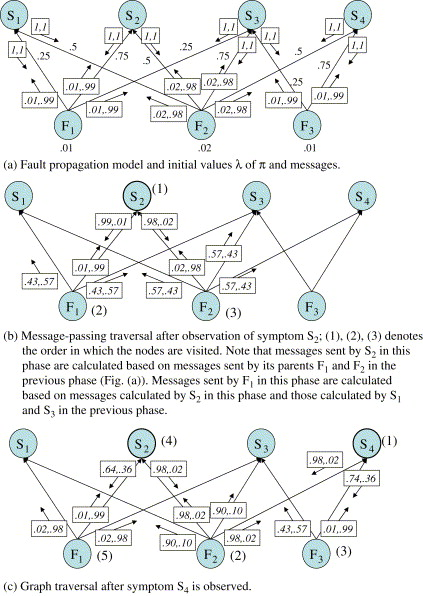
\includegraphics[width=0.5\textwidth]{Fig7}
\end{figure}

The algorithms  utilizes a message passing schema in which BN nodes exchange messages that encode certain conditional probabilities. The message that node X sends to its parent V$_j$ for every valid V$_j$'s value v$_j$ is denoted by ${\lambda}_X(v_j)$. The message that node X sends to its child U$_i$ for every valid value of X, x, is denoted by ${\pi}_{U_i}(x)$. Messages ${\lambda}_X(v_j)$ and ${\pi}_{U_i}(x)$ are calculated by node X based on messages it receives from its neighbors using the following equations (where $\beta$ is any constant and $\alpha$ is a normalizing constant)
\\
based on messages the {\it bel(x)={$\alpha$}{$\lambda$}(x){$\pi$}(x)}.

The alogirthm proceeds in an event driven manner when a symptom is observed and applying a message passing iteration traversing the graph based on an order. Figure 7 shows an example bayesian network with fault nodes F$_1$, F$_2$, F$_3$. Once the algorithm ends every node is assigned a belief probability, the probability of its existence given the symptoms. The final hypothesis is chosen using the following heuristic: (1) a most-likely fault is chosen and placed in the final hypothesis, (2) the chosen fault node is considered a part of evidence, and (4) one iteration of message passing starting from the chosen fault node is performed. Steps (1)–(3) are repeated as long as (1) the posterior distribution contains fault nodes whose probability is greater than 0.5, and (2) unexplained negative symptoms remain. An inherent property of the adapted algorithm is the capability to isolate multiple simultaneous faults even if their symptoms overlap. 

However one limitation to the modeling of the domain as bayesian network is the model has to adopt canonical models used in the literature mentioned above like noisy-OR gates, AND gates to limit the algorithm runtime to polynomial time. The comparision of different algorithms in bayesian networks is mentioned in the table 1 below.

\begin{center}
\begin{table*}[ht]
{\small
\hfill{}
    \begin{tabular}{ | c | c | c | c |}
    \hline
    Algorithm & Bucket Elimination & Iterative Belief Updating & Iterative MPE \\ \hline
    Theoretical Bound & $n^2$exp(n) & $n^5$ & $n^6$ \\ \hline
    Detection Rate & 96-100\% & 93-98\% & 95-100\% \\ \hline
    False Positive Rate & 0-4\% & 2-5\% & 0-8\% \\ \hline
    Max Network Size & 10 & 50 & 25 \\ \hline
    Algorithm iterative? & no & yes & yes \\
    \hline
    \end{tabular}}
\hfill{}
\caption{Comparision of algorithms}
\label{tb:tablename}
\end{table*}
\end{center}

\cite{Kandula:05} Shrink a tool for failrue diagnosis in IP Networks. Shrink outputs the most likely explanation for the network's faulty state –i.e., the collection of SRLGs whose failure is most likely given the IP link status. Shrink works on three modules (1) building the bayesian model (2) augemnting the model with guess edges (3) inferring the most likely explanation.

\begin{figure}[h!]
  \caption{Shrink system setup}
  \centering
    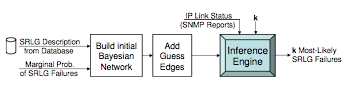
\includegraphics[width=0.5\textwidth]{Fig8}
\end{figure}

\begin{figure}[h!]
  \caption{Shrink's network model}
  \centering
    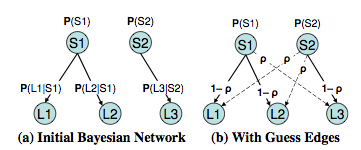
\includegraphics[width=0.5\textwidth]{Fig9}
\end{figure}

if $E_k$ denotes the event that at most k SRLGs failed within any hour, there are exactly k combinations of n possible SRLG assignmentsthat satisfy $E_k$. Given the observed link status, shrink algorithm greedily picks the most likely SRLG assignment in $E_k$; i.e., it picks $(S_1,.....,Sn)$ $\in$ $\{0,1\}^n$ such that: \\
$arg \underset{S_1,....,S_n}{max} P(S_1,.....,S_n|L_1,....L_n)$ subject to number of \{$S_i$=1\} $\leq$ k \\
There are fewer than $n^k$ value assignments in $E_k$, and for each assignment $P(S_1,...,S_n|L_1,...,L_m)$ can be computed in O(m + n) time, where m is the number of IP links and n is the number of SRLGs. So, Shrink’s running time is O($n^k$ ∗(m+n)). k=3 is a valid case for a wide range of ISP network sizes and SRLG failure probabilities and when k$\geq$3 the hypothesis performance is exponential. 

\subsection{Misc approaches}

There are several other approaches to fault localization like codebook approach which uses hamming distances to find the fault and also context free grammer which allows xpressions to be built from subexpressions, may be effectively used to represent a hierarchically organized communication system. However these are not discussed in this papaer due to the poor applicability to the real world systems and poor performance of these approaches. \cite{Calo:95}, \cite{Kliger:95}, \cite{Yemini:1996} are papers that discuss about these techiniques.

\section{Paper 1: Toward Optimal Network Fault Correction in Externally Managed Overlay Networks}
\cite{pclee:07} Paper 1 is an end-to-end approach of inferring probabilistic data-forwarding failures in an externally managed overlay network, where overlay nodes are independently operated by various administrative domains. The optimization goal is to minimize the expected cost of correcting (i.e., diagnosing and repairing) all faulty overlay nodes that cannot properly deliver data. Instead of first checking the most likely faulty nodes as in conventional fault localization problems it chooses a {\it candidate node} proceed based on a potential heuristic function and is bound to infer correctly atleast 95\% of the time.

\cite{Katzela:95}, \cite{Sethi:04} and \cite{Kandula:05} state of the art techniques that diagnose (i.e detect and localize) the components that are root causes of the network faults, however they do not focus on the {\it network fault correction} that is not only diagnosis but also considering the repair and checking costs. \cite{pclee:07} conveniently outperforms all of them and tries to derive a strategy for efficient network fault correction at minimum cost. 

Another set of research papers focus purely on the failure detection of network faults \cite{Zhuang:05}, \cite{Mizrak:05} and \cite{Avramopoulos:04} uses distributed techniques and all networks nodes to collaboratively achieve the fault detection. \cite{Avramopoulos:04} uses inspection on packets from previous hop and reports when founded corruption. The problem with this approach is that an inspection logic or monitoring points have to be setup across the network and incurs heavy costs and different administration domains prove to be obstacle in the above cases too. 

\appendix
%\bibliographystyle{abbrv}
%\bibliography{sigproc}


%
% sample.tex
% $Id: sample.tex,v 1.1 2006/03/18 00:21:36 johnh Exp johnh $
%


% The default of sigplan-proc-varsize is 9pt, indented paragraphs (acm style)
% For Sensys or other 10pt conference, use the 10pt option
%\documentclass{sigplan-proc-varsize}
% options:
%\documentclass[9pt]{sigplan-proc-varsize}
\documentclass[10pt]{sigplan-proc-varsize}
%\documentclass[noindentedparagraphs]{sigplan-proc-varsize}



% % hack to avoid the ugly ACM paragraph definition
% % => can't leave blank line after this
% (remove comment for this hack)
% \renewcommand{\paragraph}[1]{\vskip 6pt\noindent\textbf{#1 }}
\usepackage{amsmath}
\usepackage{graphicx}
\usepackage{url}
\usepackage{underscore}


\numberofauthors{1}


\author{
%
% The command \alignauthor (no curly braces needed) should
% precede each author name, affiliation/snail-mail address and
% e-mail address. Additionally, tag each line of
% affiliation/address with \affaddr, and tag the
%% e-mail address with \email.
\alignauthor Vijay Akkineni \\
        \affaddr{Department of Computer Science and Engineering}\\
        \affaddr{Georgia State University}\\
       \email{vakkineni1@student.gsu.edu}
}

\title{Fault localization in Communication Networks}

%\conferenceinfo{Phd Qualifiers'13,} {September 6, 2013, Atlanta, United States.}
%\CopyrightYear{2013}

\begin{document}

\maketitle

\begin{abstract}
This paper is about fault localization techniques in communication networks worked for Phd qualifiers examination. 
Fault Localization is an important aspect of network fault management and is a process of deducing the source of a failure from the set of observed indicatations. 
It has been an important research area in the field of networking both communication networks and wireless sensor networks.
As commuication networks grow in size and complexity it has been imposing new set of requirements on fault localization. 
Despite the amount of research done in this field we can still argue that it is an area of open for research. 
The paper essentially disucsses the work that has been done in this field in the pas few years with emphasis on the both the papers given for the examination.
\end{abstract}

% A category with the (minimum) three required fields
\category{H.4}{Communication Networks, Sensor Network Applications}{Miscellaneous}

\keywords{Fault Localization, Communication Networks, Root Cause Analysis, Causal Inference}

\section{Introduction}
  \label{sec:intro}

Fault diagnosis is an important part of networking. Faults are unavoidable in communication systems but their quick detection and isolation and repair is critical 
for the robustness, reliability and health of the system. When the networks get large and cumbersome automatic fault diagnosis and fault management is a crucial aspect.

A basic taxonomy in this field is mentioned below.

Event, defined as an exceptional condition occurring in the operation of hardware or software of a managed network, is a central concept pertaining to fault diagnosis.

Faults (also referred to as problems or root causes) constitute a class of network events that can cause other events but are not themselves caused by other 
events. Faults may be classified as: (1) permanent, (2) intermittent, and (3) transient. A permanent fault exists in a network until a repair action is taken.
Intermittent faults occur on a discontinuous and periodic basis causing a degradation of service for short periods of time.
However, frequently re-occurring intermittent faults significantly jeopardize service performance. 
Transient faults cause a temporary and minor degradation of service.

Error(Failure) is defined as a discrepancy between a computed, observed, or measured value or condition and a true, specified, or theoretically correct value or condition. 
Error is a consequence of a fault. Faults may or may not cause one or more errors. 
Errors may cause deviation of a delivered service from the specified service, which is visible to the outside world. 
Errors do not need to be directly corrected, and in many cases they are not visible externally. 
However, an error in a network device or software may cause a malfunctioning of dependent network devices or software. 
Thus, errors may propagate within the network causing failures of faultless hardware or software.

Symptoms are external manifestations of failures. They are observed as alarms—notifications of a potential failure. 
These notifications may originate from management agents via management protocol messages (SNMP trap and CMIP EVENT-REPORT), 
from management systems that monitor the network status, e.g., using command ping, system log-files or character streams sent by external equipments.

Figure 1 shows the concepts described above in an end to end perspective.

The process of fault diagnosis usually involves three steps as cited in \cite{KatzelaThesis:1996}:

\begin{itemize}
  \item Fault detection, a process of capturing on-line indications of network disorder provided by malfunctioning devices or fault detection agents in the 
  form of alarms.
  \item Fault localization (also referred to as fault isolation, alarm/event correlation, and root cause analysis) is a set of observed fault indications is analyzed to 
  find an explanation of the alarms.
  \item Testing is a process that, given a number of possible explanations, determines the actual faults.
  \item Fault Correction, by which we mean not only to diagnose, but
also to repair all faulty components within a network (This includes the testing component).
\end{itemize}

\begin{figure}[h!]
  \caption{Distinction between fault, error and symptom}
  \centering
    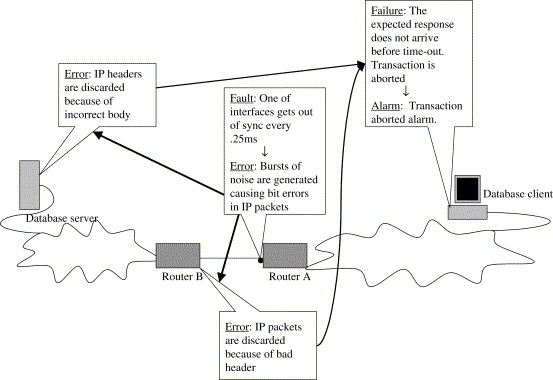
\includegraphics[width=0.5\textwidth]{Fig1}
\end{figure}

The difficulty in the fault localization process arise from the ambiguity of the observed set of alarms as same alarm can be generated from multiple different faults 
and multiple alarms can correlate back to the same fault. The incompleteness of the alarm stems from the fact that the alarm doesn't have all the information or 
there is a loss of alarm. Inconsistency among the observed alarms results from device perception of the fault is different form device to device.  

A set of alarms generated by a fault may depend on many factors such as dependencies among network devices, current configurations, services in use since 
fault occurrence, presence of other faults, values of other network parameters, etc. Due to this non-determinism the system knowledge may be subject to inaccuracy 
and inconsistency. Fault evidence may also be inaccurate because of spurious alarms, which are generated by transient problems or as a result of overly sensitive 
fault detection mechanisms. When spurious symptoms may occur, the management system may not be sure which observed alarms should be taken into account in the fault 
localization process. Event management systems should identify and eliminate multiple simultaneous related or unrelated root causes. 

In large networks distributed fault localization process should be performed in distributed fashion. Many researches \cite{Katzela:1995} and \cite{Yemini:1996} have 
concluded that distributed fault localization using a set of event management nodes is a better approach than centralized process. The complexity arised from the nature 
of error propogation, they propogate either horizontally to the peers or vertically from bottom layer to upper layers or afecting higher level services. The errors also
propogate from one management domain to a different management domain making the process even difficult. Therefore the distribution of complexity to distributed fault 
localization processes and inferring form the collective process makes the process computationally feasible and efficient. 

An alarm can insinuate different type of faults that occurred in different communication devices where in fault localization process may not comeup with a 
definitive answer. Few approaches that will be discussed in this paper combine fault localization with testing and fault ocrrection process to validate the hypothesis. 
Therefore there should be some kind of optimality measure or confidence measure that should be employed in measuring the hypothesis that the localization process 
came up with and it could include the lowest cost or min failure probability or some heuristic function which optimizes the process of validating the hypothesis.

Numerous works have been proposed on fault localization process. The techniques are dervice from different areas of artificial intelligence, graph theory, 
neural networks, automata theory and many other approaches. Figure 2 broadly classifies the exisiting solutions. The two papers provided for the exam falls into the 
category of end to end testing scenarios and proababilistic reasoning and derive their roots from bayesian network analysis. 

\begin{figure}[h!]
  \caption{Classification of fault localization techniques}
  \centering
    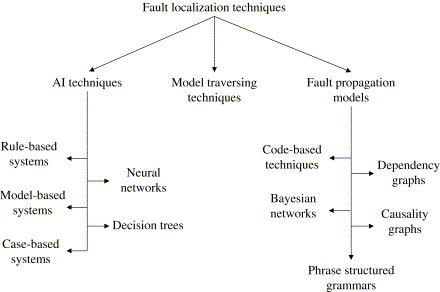
\includegraphics[width=0.5\textwidth]{Fig2}
\end{figure}

This paper presents the background research that has been done before paper 1 in section 2 - 4 and in section 5 presents the paper 1 \cite{pclee:07}.

\section{Expert Systems techniques}
Most widely used technique in the field of fault localization and diagnosis are expert systems as they try to mimic the actions of human expert. 
Most expert systems use rule based system as their inference engine. \cite{Peng:97},\cite{Liu:99} and \cite{Nygate:95} are examples of expert systems.

The expert systems developed differ in the knowledge they use. Rule based fault localization solely depend on the 
structure of the knowledge base as rule definition language. In \cite{Lor:93}   the knowledge base is divided to reusable 
knowledge modeled as core knowledge and customized knowledge.  in  \cite{Liu:99} the rules are organized as composite events and 
an intervention of human expert is required to update the event base.  The rule based systems can act as a powerful tool to eliminate 
least likely hypothesis. Although the RBR paradigm is appropriate for problem-solving tasks that are confined and well-understood its limitations are.

\begin{itemize}
  \item an in-ability to learn from experience.
  \item Fan inability to deal with novel problems.
  \item the difxulty of updating the systems to keep up with rapidiy changing domains such as expanding heterogeneous network.
\end{itemize}

in Model bases expert systems like \cite{Nygate:95} conditions are ususally accosiated with rules which includes predicates referring to system model. 
These predicates test the syetem for existence of relationship among system component. \cite{Nygate:95} 
uses correlation tree skeletons describing cause and effect relation ships between event. regardless of what expert system is being used localization process is 
always driven by inference engine and correaltion rules between events. 

\cite{Lewis:93} and \cite{Gardner:96} are examples of Case-based reasoning systems. The goals of CBR systems are (i) to learn from experience, (ii) to 
offer solutions to novel problems based on past experience, and (iii) to avoid expensive maintenance. The basic idea of CBR is to recall, adapt, and 
execute episodes of former problem-solving in an attempt to deal with a current problem. Former episodes of problem-solving are represented as cases in a case 
library. When confronted with a new problem, a CBR system retrieves a similar case and tries to adapt the case in an attempt to solve the outstanding problem. 
The disadvantages of such a system is the time complexity in retrieving a case that is the closest match to the event and the close tailoring of the application 
to the domain.

In addition to the above mentioned techniques there are other notable techniques are neural networks based approaches \cite{Gardner:97} \cite{Gardner:98} and 
decision tree based approaches \cite{Rodosek:98}. Neural networks have parallel computing architecture and are very fast avoiding bottlenecks which 
commonly arises from serial processing. But the main disadvantage is that the learning process requires intesive training  and in communication networks 
where all the alarms signatures are not readily available for pattern recognition.

Decision tree aproaches are simple and allows expressive representation of expert knowledge howeever they are limited by the dependencies sepcific 
applications nad degraded accuracy in noisy scenarios \cite{Russell:96} \cite{Koller:10}.

\section{Model traversing techniques}
\cite{Katker:96}, \cite{Katker:971}, \cite{Katker:97} and \cite{Gruschke:98} are all Model Traversing that use formal representation of communication 
system with clearly marked relationships across network entities. This technique identifies faults by traversing a model of entities starting form the entity whic reported an alarm and also involves a fault identification process to identify and locate faulty network entities.

The model representation used by this technique is object-oriented representation of the given system. It is based on the OSI management framework and uses GDMO (Guidelines for  Definition  of Managed Objects) with extensions to the MO to model dependencies and services between the entities. This approach can make automated testing possible which can test for various testing entities availability and quality of service standards. 

The event correlation in model traversing techniques is event driven as when an event occurs it is being mapped to the reported entity and the managed object representing that entity. For every event the search begins from the MO reporting the event and is searched recursively forllowing all relationship links between MO's using fault localization algorithms.  Fault localization algorithms used in this technique can be of various flavours.  models every event as singleton classes and merges them whenever they are traced to the same node. Typical proerties of such techniques involve 

\begin{itemize}
  \item Level at which a particular fault has occurred in the model.
  \item Event Type.
  \item Event severity.
  \item Event Origin - to identify if the event occurred is primary or secondary.
\end{itemize}

\begin{figure}[h!]
  \caption{Architecture of a model traversing technique prototype}
  \centering
    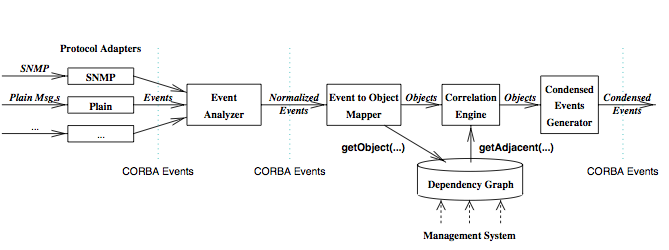
\includegraphics[width=0.5\textwidth]{Fig3}
\end{figure}

The MO's provide functions which lets the process test the entity for its operational status.  The root cause is found when the process stops at an entity and validates that it is a malfucntioning object and doesn't depend on any other object. In a multi layer model vertical search is performed first and then horizontal search in the next lower layer to check its peer at the end of search process votes are collected to identify the faulty elements and the device that recieves the most votes is declared faulty and a testing process kicks in to test the validity of the hypothesis. 

Model traversing techniques are pretty robust agianst network configuration changes and very useful in the scenario's where automated testing is a requirement and the depedency model is very natural as they are modeled as Trees or Graphs. 

The biggest drawback is the Fault Propagation Patterns and when there  fault is a logical combination of multiple devices and byzatine problems. It also incurs heavy testing costs. 

\section{Graph-theoretic techniques}
 
Grap theoretic techniques depend on gaphical model of a system called fault proppagation model(FPM). FPM represents fault and symptoms that occur in a system. 
The symptoms that are observed are mapped into nodes in the FPM and localization algorithms analyze the graph to infer the best explanation of the observed symptoms. 

These techniques require a knowlede of depedencies among the abstract and physical system components and how these failures in one component are related to 
other components. The success of the fault localiztion algorithm depends on the the accuracy of this a priori specification.

FPM's are genrally modeled as (i) Cuasaultiy graph is is a DAG whose nodes are events and edges represent the causality implications i.e cause effect relationships 
between events. They are carry probabilties to the nodes and edges implying the probability of a certain event to happen. 
Dependency Graph is a directed graph {\it{G=(O,D)}} where O represent a finite set of nodes and D are the depedency edges between Objects. 
The directed edge (o$_{i}$,o$_{j}$) $\in$ D represents that when o$_{i}$ fails o$_{j}$ fails or emits some kind of error. 
The edges are also labeled with conditional probabilities. Figure 4 represents such a depedency graph.

\begin{figure}[h!]
  \caption{A Network example along with the dependecy graph \cite{Katzela:95}}
  \centering
    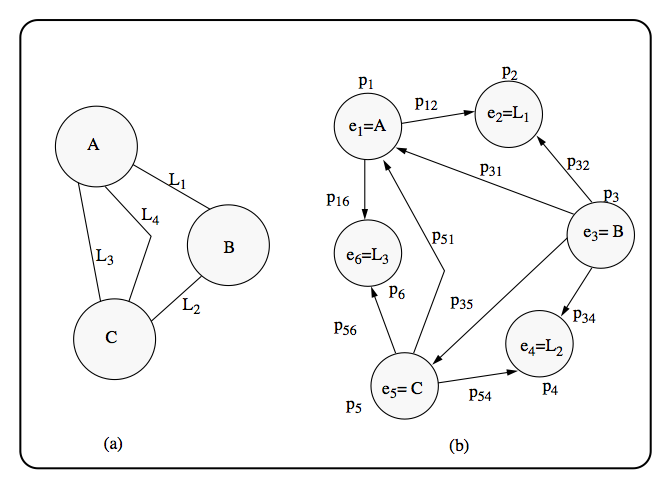
\includegraphics[width=0.5\textwidth]{Fig4}
\end{figure}

A lot of approaches using dependency graph, a critical assumption involves that an entity may fail in only one way. If that is the case the causal graph and dependecy graph would be the same.  In the case of multiple failures associated to a single entity they can be divided into sets such as {\it{complete failure, abnormal transmission delay, high packet loss, etc.}}. The dependecy graph in this case would have multiple edges between failure modes and the Object(entity). Sethi et all in \cite{Sethi:02}, \cite{Sethi:041}, \cite{Sethi:04} have modeled using multiple failure modes principle. 

A fault localalization algorithm, based on the provided FPM generally returns a number of hypothesis that best explain the observed symptoms. The problem of finding best explanation of the recieved alarms is {\it{NP-hard}} problem and proved in \cite{Katzela:95} by reducing the given problem to a Min Set-Cover problem.

\subsection{Divide and conquer algorithm}
The divide and conquer algorith uses a FPM assuming that one type of failure is allowed per object. It is a window based technique i.e gathers all the faults in a time window and analyzes them. 

System model is a directed graph G = ( E ,D) called the dependencygraph, where E is a finite nonempty set of active terminal objects e$_i$, and a directed edge (e$_i$, e$_j$) $\in$ D denotes the fact that a fault in e$_i$ has a side effect on e$_j$ i.e., e$_j$ is dependent on e$_i$.
Each vertex e$_i$ is assigned a weight p$_i$ that is the probability that the object e$_i$ fails independently of the state (failed or not failed) of any other active terminal object that is dependent on it. Each directed edge ( e$_j$,e$_i$) is assigned a weight p$_{ji}$ which represents the strength of dependency between the entities it connects. Specifically, p$_{ji}$ , is the conditional probability p$_{ji}$ = P(e$_j$ fails\textbar e$_i$ fails) that entity e$_j$, fails as a result of the failure of entity e$_i$. In addition, the weight of a directed path is defined as the product of all the weights of the edges that compose the path. Finally, the strength of dependency p$_{kl}$ between two non-adjacent vertices e$_k$ and e$_l$, is defined as the maximum of the weights of all directed paths from e$_k$ to e$_l$.

Let D(a$_i$) for every a$_i$ alarm be the domain of alarms that defines as the set of objects that might have caused the alarm.  The domain of an alarm calculation is a variation of single source problem that finds the min cost paths from a source vertex to all other graphs and the nodes are chosen such that the cost of path e$_i$ to e$_j$ is subject to restriction that we include only the minimum cost paths with cost $\leq$ log(W) where W is a parameter.

The outline of the algorithm run has been given below.

\begin{itemize}
  \item Start with the set S of objects associated with the alarm cluster.
  \item Find the partitioning of the set S resulting in two disjoint sets so in each set the objects exhibit the maximum mutual dependency, i.e., for every object e$_i$ and e$_j$, that belongs to the same set and e$_k$ that does not belong to the set, the dependency weight p$_{ij}$is greater than the dependency weights p$_{ik}$, p$_{ki}$, p$_{jk}$, p$_{kj}$.
  \item Of the two sets, select the one that explains all the received alarms and has the maximum probability that at least one of the entities in the set is a fault. If there is no such set then find the subset of alarms that each set explains and select both.
  \item Apply the previous two steps of the algorithm recursively to the selected sets until the resulting sets of the current partitioning are singletons.
\end{itemize}

By partitioning with the maximum mutual dependency criterion we group together objects that are highly dependent on each other and when the result of partitionining, both the sets are capable of explaingin all the alarms then we select one set that has higher probability of having one of them at fault. 

When determining atleast on memeber of the subset is faulty it is calcualted using. 

P(S) = ${\underset{\forall i:e_i \in S}{\sum}}[p_i + \underset{\forall j:e_j \in S , j \neq i}{\sum} p_{ij}.p_j]$


\begin{figure}[h!]
  \caption{Divide and Conquer algorithm \cite{Katzela:95}}
  \centering
    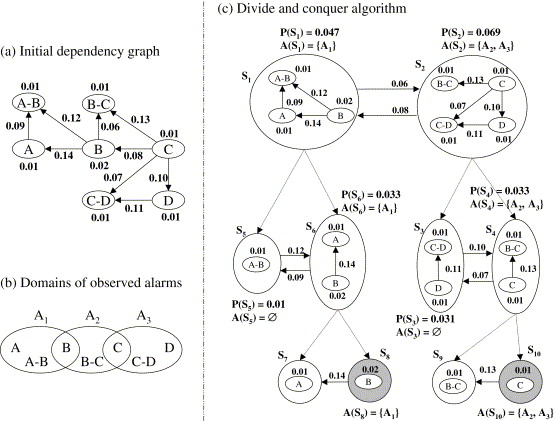
\includegraphics[width=0.5\textwidth]{Fig5}
\end{figure}

In algorithm runs in two phases where in the first phase algorithm finds the maximum mutual partitionings of the entities in the set S. The result of Phase I is a hierarchical clustering of the entities in the set S. In the Phase II a fault localization algorithm is recursively invoked to find the subsets that are supposed to be used. The first subcluster contains all alarms that may be explained using the subset with the higher probability that one of its members was a primary source of a failure. The second subcluster contains the remaining alarms from the original alarm cluster. Its domain is the other of the two subsets. The recursive procedure is then invoked twice, taking the two subclusters and their respective domains as parameters. The recursion continues until the input alarm cluster domain is a singleton. 

The algorithm mentioned above gives the explanation of the observed alarms but may not prouce the best output as it is a approximation algorithm based on maximum mutual dependency heuristic. The runtime complexity of the algorithm is O(N$^{3}$) and the partitioning phase runtime is O(logN). The drawback of the algorithm is it cannot handle the lost or spurious alarms and is a time window based determinsitic algorithm.

\subsection{Bayesian Reasoning approach}
Bayesian network or probabilistic graphical model represents a set of random varaibles and their conditional dependencies using a directed acyclic graph. In the context of fault localization the random variables represent the state of network entities and the occurrence of network events. 

\begin{figure}[h!]
  \caption{A example bayesian network}
  \centering
    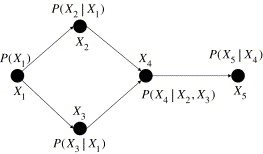
\includegraphics[width=0.5\textwidth]{Fig6}
\end{figure}

Belief networks are used to make four basic queries given evidence set e: belief assessment, most probable explanation, maximum a posteriori hypothesis, and maximum expected utililty \cite{Pearl:98}

\cite{Cynthia:97}, \cite{Sethi:02}, \cite{Sethi:041} and \cite{Sethi:04} all the papers try to model the FPM as a bayesian network using a layered fault model apparoach and in general fault component models are divided into services, protocols and functions. The recursive dependencies between services, protocols and functions constitue a dependenct graph. Uncertainty about dependencies between communication system entities is represented by assigning probabilities to the links and/or nodes in the dependency or causality graph. 

The queries for belief assesment and most probable explanation are of particular interest in the approaches mentioned above. The belief assesment task is to compute $bel(V_i=v_i) = P(V_i=v_i|e)$. given an evidence e, {\it bel}  gives the certainity of an event happening under the evidence. The most probable explanation task is to find an assignment that best explains the observed evidence e, i.e.,  \\
$P(A_{max}) = max_A \underset{i=1}{\overset{n}{\pi}} P(V_i=v_i^A | Par(V_i)^A)$ \cite{Pearl:98}. \\
It is known that the above tasks are NP-{\it hard} in the regular belief networks. A belief updating algorithm, polynomial with respect to $|$V$|$, is available for {\it polytrees}, i.e., directed graphs without undirected cycles. The exact calculation of the best explanatory hypothesis requires a number of steps that is exponential with respect to the number of graph nodes. One of the most popular exact algorithms bucket elimination is used as a reference algorithm against {\it iterative belief updating} algorithm and {\it iterative MPE query} algorithm.

\begin{figure}[h!]
  \caption{Bayesian Network message passing algorithm example}
  \centering
    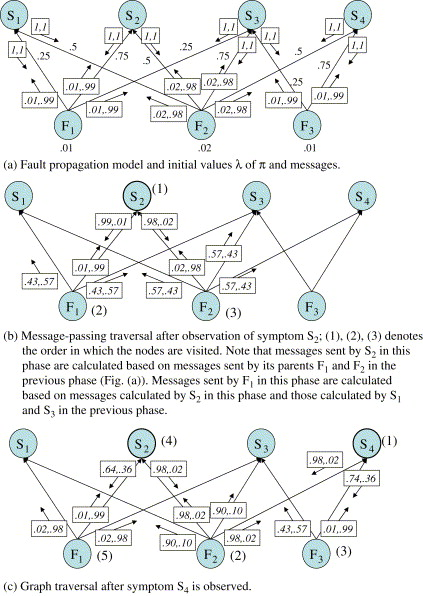
\includegraphics[width=0.5\textwidth]{Fig7}
\end{figure}

The algorithms  utilizes a message passing schema in which BN nodes exchange messages that encode certain conditional probabilities. The message that node X sends to its parent V$_j$ for every valid V$_j$'s value v$_j$ is denoted by ${\lambda}_X(v_j)$. The message that node X sends to its child U$_i$ for every valid value of X, x, is denoted by ${\pi}_{U_i}(x)$. Messages ${\lambda}_X(v_j)$ and ${\pi}_{U_i}(x)$ are calculated by node X based on messages it receives from its neighbors using the following equations (where $\beta$ is any constant and $\alpha$ is a normalizing constant)
\\
based on messages the {\it bel(x)={$\alpha$}{$\lambda$}(x){$\pi$}(x)}.

The alogirthm proceeds in an event driven manner when a symptom is observed and applying a message passing iteration traversing the graph based on an order. Figure 7 shows an example bayesian network with fault nodes F$_1$, F$_2$, F$_3$. Once the algorithm ends every node is assigned a belief probability, the probability of its existence given the symptoms. The final hypothesis is chosen using the following heuristic: (1) a most-likely fault is chosen and placed in the final hypothesis, (2) the chosen fault node is considered a part of evidence, and (4) one iteration of message passing starting from the chosen fault node is performed. Steps (1)–(3) are repeated as long as (1) the posterior distribution contains fault nodes whose probability is greater than 0.5, and (2) unexplained negative symptoms remain. An inherent property of the adapted algorithm is the capability to isolate multiple simultaneous faults even if their symptoms overlap. 

However one limitation to the modeling of the domain as bayesian network is the model has to adopt canonical models used in the literature mentioned above like noisy-OR gates, AND gates to limit the algorithm runtime to polynomial time. The comparision of different algorithms in bayesian networks is mentioned in the table 1 below.

\begin{center}
\begin{table*}[ht]
{\small
\hfill{}
    \begin{tabular}{ | c | c | c | c |}
    \hline
    Algorithm & Bucket Elimination & Iterative Belief Updating & Iterative MPE \\ \hline
    Theoretical Bound & $n^2$exp(n) & $n^5$ & $n^6$ \\ \hline
    Detection Rate & 96-100\% & 93-98\% & 95-100\% \\ \hline
    False Positive Rate & 0-4\% & 2-5\% & 0-8\% \\ \hline
    Max Network Size & 10 & 50 & 25 \\ \hline
    Algorithm iterative? & no & yes & yes \\
    \hline
    \end{tabular}}
\hfill{}
\caption{Comparision of algorithms}
\label{tb:tablename}
\end{table*}
\end{center}

\cite{Kandula:05} Shrink a tool for failrue diagnosis in IP Networks. Shrink outputs the most likely explanation for the network's faulty state –i.e., the collection of SRLGs whose failure is most likely given the IP link status. Shrink works on three modules (1) building the bayesian model (2) augemnting the model with guess edges (3) inferring the most likely explanation.

\begin{figure}[h!]
  \caption{Shrink system setup}
  \centering
    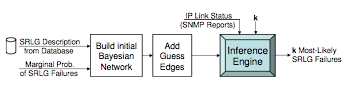
\includegraphics[width=0.5\textwidth]{Fig8}
\end{figure}

\begin{figure}[h!]
  \caption{Shrink's network model}
  \centering
    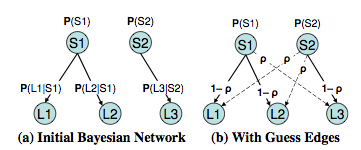
\includegraphics[width=0.5\textwidth]{Fig9}
\end{figure}

if $E_k$ denotes the event that at most k SRLGs failed within any hour, there are exactly k combinations of n possible SRLG assignmentsthat satisfy $E_k$. Given the observed link status, shrink algorithm greedily picks the most likely SRLG assignment in $E_k$; i.e., it picks $(S_1,.....,Sn)$ $\in$ $\{0,1\}^n$ such that: \\
$arg \underset{S_1,....,S_n}{max} P(S_1,.....,S_n|L_1,....L_n)$ subject to number of \{$S_i$=1\} $\leq$ k \\
There are fewer than $n^k$ value assignments in $E_k$, and for each assignment $P(S_1,...,S_n|L_1,...,L_m)$ can be computed in O(m + n) time, where m is the number of IP links and n is the number of SRLGs. So, Shrink’s running time is O($n^k$ ∗(m+n)). k=3 is a valid case for a wide range of ISP network sizes and SRLG failure probabilities and when k$\geq$3 the hypothesis performance is exponential. 

\subsection{Misc approaches}

There are several other approaches to fault localization like codebook approach which uses hamming distances to find the fault and also context free grammer which allows xpressions to be built from subexpressions, may be effectively used to represent a hierarchically organized communication system. However these are not discussed in this papaer due to the poor applicability to the real world systems and poor performance of these approaches. \cite{Calo:95}, \cite{Kliger:95}, \cite{Yemini:1996} are papers that discuss about these techiniques.

\section{Paper 1: Toward Optimal Network Fault Correction in Externally Managed Overlay Networks}
\cite{pclee:07} Paper 1 is an end-to-end approach of inferring probabilistic data-forwarding failures in an externally managed overlay network, where overlay nodes are independently operated by various administrative domains. The optimization goal is to minimize the expected cost of correcting (i.e., diagnosing and repairing) all faulty overlay nodes that cannot properly deliver data. Instead of first checking the most likely faulty nodes as in conventional fault localization problems it chooses a {\it candidate node} proceed based on a potential heuristic function and is bound to infer correctly atleast 95\% of the time.

\cite{Katzela:95}, \cite{Sethi:04} and \cite{Kandula:05} state of the art techniques that diagnose (i.e detect and localize) the components that are root causes of the network faults, however they do not focus on the {\it network fault correction} that is not only diagnosis but also considering the repair and checking costs. \cite{pclee:07} conveniently outperforms all of them and tries to derive a strategy for efficient network fault correction at minimum cost. 

Another set of research papers focus purely on the failure detection of network faults \cite{Zhuang:05}, \cite{Mizrak:05} and \cite{Avramopoulos:04} uses distributed techniques and all networks nodes to collaboratively achieve the fault detection. \cite{Avramopoulos:04} uses inspection on packets from previous hop and reports when founded corruption. The problem with this approach is that an inspection logic or monitoring points have to be setup across the network and incurs heavy costs and different administration domains prove to be obstacle in the above cases too. 

Paper1 considers and end-end inference approach using end-end measurements, infers components that are faulty in forwarding data. This applies perfectly to the scenario like CAN\cite{Ratnasamy:01} and CHORD\cite{Stoica:01} where each overlay node builds a routing tree with itself as a root and in this setting every root to leaf path is monitored to find faulty path and anamolous behaviours on the path. One anamoulous behaviour could be number of correct packets bot being delivered in a fixed time period, such a validation could prove to be very important in QOS factor.  The authors are particular interested in diagonize and repairing faulty nodes in overlay networks like RON\cite{Andersen:01}, SON\cite{Duan:03} and SOS\cite{Misra:04}. The proposed fault correction mechanism suits well to this type of  networks. 

\subsection{Problem Formulation}
\cite{pclee:07} considers a logical tree as T=$(N,\{{p_i}\},\{{c_i}\}),$ where N is the set of overlay nodes, $p_i$ is the failure probability of node i$\in$N, and $c_i$ is the checking cost of deciding if node i$\in$N is faulty. Overlay set node N provides a topology information and sequence of nodes. The construction of failure probabilities and cost probabilities depend on Failure model and Cost model.

{\bf Failure Model} focus on the nodes that cannot forward data or fails to comply with a QOS because of which packets get dropped or fails to get delivered. Focus mainly stands on fail-stop failues like power outages, full transmission queues, hardware errors and route misconfigurations. The failure probabilities are calculated using statistical measurements of reliability indexes of node elements(vulnerability modelling).  Authors also performed analysis of the  mechanism under inaacurate probabilities and is provide in the results section of this paper. Important consideration to be made is that failure probabilities of nodes are independent of each other. 

{\bf Cost Model} provides the checking costs using personnel hours, wages and time effort that goes into debugging the problem or even the cost of the equipment. Important cirteria to be noted in the cost model the repair costs are not conisdered as eventually every fault has to be repaired. $p_i$ and $c_i$ can be any values between [0,1] and [0,$\infty$].

Each node in a logical tree T is classified as fault or non-faulty. and definitions are being made on each root to leaf path that exhibits an anamalous behaviour. Since an end-to-end inference mechanism is being made we only know that something is wrong with the path rather than which node is at fault. Each node in T is referred to as {\it bad} if it is faulty and {\it good} if it is non-faulty and a path in T is bad if it has atleast one {\it bad} node. An important consideration is that the node behaviour remains the same across all the paths as only fail-stop considerations are being made. 

Given a logical tree T we can infer the good path and bad paths by end to end inference mechanism, for example root can send a probe and collect all measurement results. We now create a bad Tree by pruning of all the good paths form the logical tree and also call it T with abuse of notation. Bad tree now becoms input to the inference algorithm which determines which set of nodes to be corrected(checked and repaired).

The optimization goal of this paper is to minimize the expected cost of correcting all faulty nodes in a given tree. repairing cost is not considered as eventually all the nodes have to be repaired and any strategy that is employed will eventually correct all the nodes. Here we focus only on the sequential case as checking the nodes in parallel doesnt improve the total expected checking cost so the inference algorithm only return one single node that is supposed to be the best node to check first. The best node is the first node that is from a diagnostic sequence {\it S} = $\{l_1,l_2,....,l_N\}$ and gives us {\it N!} diagnositic sequences.

When a particular node {\it $l_i$} lies on a bad path we do no know whether it is a good node or a bad node but if it is on a good node we know for sure it is a good node. {\it $l_i$}  gets {\it checked or skipped} based on the examination of the node. Thus we can summarize the total cost of checking a tree {\it T} is given by  \\
$\underset{i=1}{\overset{|N|}{\sum}} c_{l_i} Pr(node\ l_i\ is\ checked\ | \ nodes\ l_1,...,l_{i-1}\ known\ to\ be\ good)$ \\
So the best node would be the first node in the diagnosis sequence and the inference works on the current topolgy to indetify this node and when the node is corrected the revised topology is fed into the inference algorithm to output the next node. The total complexity of calculating the expected cost of a diganosis sequence is O($n^3$) and since there are n! differenct sequences, the brute force approach has a complexity of O($n^3$n!). The complexity and the way to calculate the total cost for the diagnostic sequence is mentioned in Appendix A of \cite{pclee:07}. In the interest of space and lenth only the highights are being mentioned here.

{\bf Conditional Failure Probabilties}: the nodes in T by 1 to $|$N$|$ in breadth- first-search order. $T_i$ is the subtree rooted at node i. $C_i$ is the set such that k$\in$$C_i$ if node k is a   child node of {\it i}. thus conditional failure probability is given by bayesian probability rule where Pr($X_i$) is the independent failure probability of a node, and Pr($T_1$) is the probability of the tree is bad at root, $Pr(T_1|X_i)$ is the probability that a tree is a bad tree upon the event that a node is bad. \\
$Pr(X_i|T_1) = \frac{Pr(T_1|X_i)Pr(X_i)}{Pr(T_1)}$ by baye's rule.\\
where\\
$Pr(T_i) = p_i+(1-p_i) \underset{k{\in}C_i}{\pi}Pr(T_k) , \forall i \in [1,|N|]$\\
\\

\[
 Pr(T_i|X_j) =
  \begin{cases}
   Pr(T_i) & \text{if } i > j \\
   1       & \text{if } i=j \\
   p_i+(1-p_i)  \underset{k{\in}C_i}{\pi} Pr(T_k|X_j)  & \text{if } i<j
  \end{cases}
\] \\

The idea here is that a subtree $T_i$ is bad if either the node itself is bad or node {\it i} is good and the subtree rooted at {\it i} is bad. Using dyanmic programming the above equation can be computed in O($N^2$) which is the conditional failure probabitlity of a node. 

{\bf Expected Cost of  a Diagnosis Sequence}: Let ${T_{l_i}}^D$ be the event that the subtree rooted at node ${l_i}$ is a bad tree after nodes ${{l_1},...,{l_{i-1}}}$ have been examined (i.e., checked or skipped). Let ${A_{l_i}}^D$ be the event that every ancestor j of node ${l_i}$, such that j $\in\{l_{i+1},...,l_{|N|}\}$ (i.e., node j is examined after node ${l_i}$), is a good node. Since every node is examined in a sequential way in the diagnosis sequence, when $l_i$ is examined, nodes $l_1,....,l_{i-1}$ have been examined and they are good. Thus, \\
$Pr({T_{l_i}}^D) = Pr(T_{l_i}|p_{l_1}= ... = p_{l_{i-1}} = 0)$, and \\
$Pr({A_{l_i}}^D) = Pr(A_{l_i}|p_{l_1}= ... = p_{l_{i-1}} = 0)$ \\
Where $T_{l_i}$ is the event that the subtree rooted at node $l_i$ is bad, and $A_{l_i}$ is the event that all ancestors of node $l_i$ are good. If the subtree rooted at node $l_i$ remains a bad tree or at least one of the ancestors of node $l_i$ is a bad node, then node $l_i$ still lies on bad path and needs to be checked. Thus, \\
$ Pr(node\ l_i\ is\ checked| T, nodes\ l_1,...,l_{i-1} known\ to\ be\ good)$ \\
$=Pr({T_{l_i}}^D \cup \neg{{A_{l_i}}^D} | T)$\\
Thus the expected cost of S given that T is a bad tree is: \\
\center$ \underset{i=1}{\overset{n}{\sum}} c_{l_i} Pr({T_{l_i}}^D \cup \neg{{A_{l_i}}^D} | T)$\\
Brute force algorithm which inspects all the sequences is given in figure 10. This algorithm makes a good reference for comapring against the heuristic based ones.

\begin{figure}[h!]
  \caption{Bruce Force Algorithm}
  \centering
    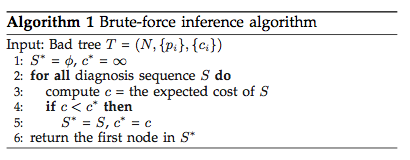
\includegraphics[width=0.5\textwidth]{Fig10}
\end{figure}

\subsection{Naive Heuristics for Inference Algorithm}
Intuitively the best node returned by the inference algorithm can be either based on the highest conditional failure probabiltiy or checking cost.  The authors provided a simple counter example in which neither the selection of node based on conditional failure probability nor the one selected based on checking cost gave the optimal solution. The three heuristics authors chose naively are (1) {\it Naive_Prob} (2) {\it Naive_Cost} (3) {\it Naive_Prob_Cost} . Based on the experimental setup where a 200 bad trees are tested with the three heuristic mentioned above with varying probabiltiy and cost distributions. Depending on the distributions of $p_i$ and $c_i$, the proportion of instances where the best choice is made can be as low as 10\% for Naive-Prob and Naive-Cost  and less than 55\% for Naive-Prob-Cost.
\begin{figure}[h!]
  \caption{Naive-Prob, Naive-Cost, and Naive-Prob-Cost performance}
  \centering
    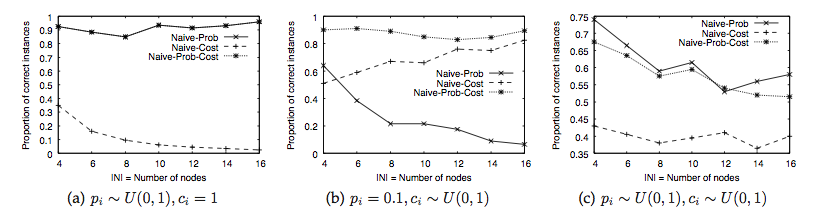
\includegraphics[width=0.5\textwidth]{Fig11}
\end{figure}

\subsection{Candidate Node}
The authors show that instead of selecting a node to test based on naive choices we should select a {\it candidate node} based on the maximization of a {\it potential function}. Let $A_i$ be the event that the ancestors of node {\it i} are all good. If node {\it r} is the root node, then we let $A_r$ be always true and $Pr(A_r) = 1$. The potential of a candidate node is calculated using the formula. \\
                        \center $\phi({\it i,T)} = \frac{Pr(T|X_i,A_i)p_i}{c_i(1-p_i)}$
\appendix
%\bibliographystyle{abbrv}
%\bibliography{sigproc}


%
% sample.tex
% $Id: sample.tex,v 1.1 2006/03/18 00:21:36 johnh Exp johnh $
%


% The default of sigplan-proc-varsize is 9pt, indented paragraphs (acm style)
% For Sensys or other 10pt conference, use the 10pt option
%\documentclass{sigplan-proc-varsize}
% options:
%\documentclass[9pt]{sigplan-proc-varsize}
\documentclass[10pt]{sigplan-proc-varsize}
%\documentclass[noindentedparagraphs]{sigplan-proc-varsize}



% % hack to avoid the ugly ACM paragraph definition
% % => can't leave blank line after this
% (remove comment for this hack)
% \renewcommand{\paragraph}[1]{\vskip 6pt\noindent\textbf{#1 }}
\usepackage{amsmath}
\usepackage{graphicx}
\usepackage{url}
\usepackage{underscore}


\numberofauthors{1}


\author{
%
% The command \alignauthor (no curly braces needed) should
% precede each author name, affiliation/snail-mail address and
% e-mail address. Additionally, tag each line of
% affiliation/address with \affaddr, and tag the
%% e-mail address with \email.
\alignauthor Vijay Akkineni \\
        \affaddr{Department of Computer Science and Engineering}\\
        \affaddr{Georgia State University}\\
       \email{vakkineni1@student.gsu.edu}
}

\title{Fault localization in Communication Networks}

%\conferenceinfo{Phd Qualifiers'13,} {September 6, 2013, Atlanta, United States.}
%\CopyrightYear{2013}

\begin{document}

\maketitle

\begin{abstract}
This paper is about fault localization techniques in communication networks worked for Phd qualifiers examination. 
Fault Localization is an important aspect of network fault management and is a process of deducing the source of a failure from the set of observed indicatations. 
It has been an important research area in the field of networking both communication networks and wireless sensor networks.
As commuication networks grow in size and complexity it has been imposing new set of requirements on fault localization. 
Despite the amount of research done in this field we can still argue that it is an area of open for research. 
The paper essentially disucsses the work that has been done in this field in the pas few years with emphasis on the both the papers given for the examination.
\end{abstract}

% A category with the (minimum) three required fields
\category{H.4}{Communication Networks, Sensor Network Applications}{Miscellaneous}

\keywords{Fault Localization, Communication Networks, Root Cause Analysis, Causal Inference}

\section{Introduction}
  \label{sec:intro}

Fault diagnosis is an important part of networking. Faults are unavoidable in communication systems but their quick detection and isolation and repair is critical 
for the robustness, reliability and health of the system. When the networks get large and cumbersome automatic fault diagnosis and fault management is a crucial aspect.

A basic taxonomy in this field is mentioned below.

Event, defined as an exceptional condition occurring in the operation of hardware or software of a managed network, is a central concept pertaining to fault diagnosis.

Faults (also referred to as problems or root causes) constitute a class of network events that can cause other events but are not themselves caused by other 
events. Faults may be classified as: (1) permanent, (2) intermittent, and (3) transient. A permanent fault exists in a network until a repair action is taken.
Intermittent faults occur on a discontinuous and periodic basis causing a degradation of service for short periods of time.
However, frequently re-occurring intermittent faults significantly jeopardize service performance. 
Transient faults cause a temporary and minor degradation of service.

Error(Failure) is defined as a discrepancy between a computed, observed, or measured value or condition and a true, specified, or theoretically correct value or condition. 
Error is a consequence of a fault. Faults may or may not cause one or more errors. 
Errors may cause deviation of a delivered service from the specified service, which is visible to the outside world. 
Errors do not need to be directly corrected, and in many cases they are not visible externally. 
However, an error in a network device or software may cause a malfunctioning of dependent network devices or software. 
Thus, errors may propagate within the network causing failures of faultless hardware or software.

Symptoms are external manifestations of failures. They are observed as alarms—notifications of a potential failure. 
These notifications may originate from management agents via management protocol messages (SNMP trap and CMIP EVENT-REPORT), 
from management systems that monitor the network status, e.g., using command ping, system log-files or character streams sent by external equipments.

Figure 1 shows the concepts described above in an end to end perspective.

The process of fault diagnosis usually involves three steps as cited in \cite{KatzelaThesis:1996}:

\begin{itemize}
  \item Fault detection, a process of capturing on-line indications of network disorder provided by malfunctioning devices or fault detection agents in the 
  form of alarms.
  \item Fault localization (also referred to as fault isolation, alarm/event correlation, and root cause analysis) is a set of observed fault indications is analyzed to 
  find an explanation of the alarms.
  \item Testing is a process that, given a number of possible explanations, determines the actual faults.
  \item Fault Correction, by which we mean not only to diagnose, but
also to repair all faulty components within a network (This includes the testing component).
\end{itemize}

\begin{figure}[h!]
  \caption{Distinction between fault, error and symptom}
  \centering
    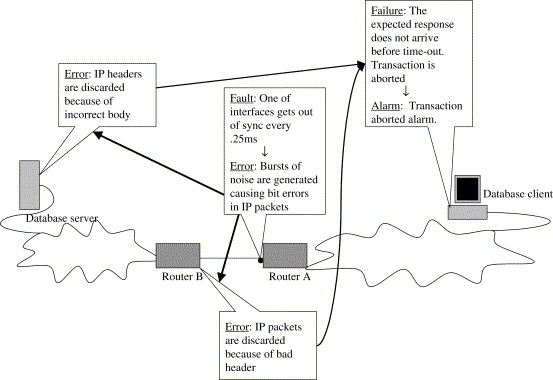
\includegraphics[width=0.5\textwidth]{Fig1}
\end{figure}

The difficulty in the fault localization process arise from the ambiguity of the observed set of alarms as same alarm can be generated from multiple different faults 
and multiple alarms can correlate back to the same fault. The incompleteness of the alarm stems from the fact that the alarm doesn't have all the information or 
there is a loss of alarm. Inconsistency among the observed alarms results from device perception of the fault is different form device to device.  

A set of alarms generated by a fault may depend on many factors such as dependencies among network devices, current configurations, services in use since 
fault occurrence, presence of other faults, values of other network parameters, etc. Due to this non-determinism the system knowledge may be subject to inaccuracy 
and inconsistency. Fault evidence may also be inaccurate because of spurious alarms, which are generated by transient problems or as a result of overly sensitive 
fault detection mechanisms. When spurious symptoms may occur, the management system may not be sure which observed alarms should be taken into account in the fault 
localization process. Event management systems should identify and eliminate multiple simultaneous related or unrelated root causes. 

In large networks distributed fault localization process should be performed in distributed fashion. Many researches \cite{Katzela:1995} and \cite{Yemini:1996} have 
concluded that distributed fault localization using a set of event management nodes is a better approach than centralized process. The complexity arised from the nature 
of error propogation, they propogate either horizontally to the peers or vertically from bottom layer to upper layers or afecting higher level services. The errors also
propogate from one management domain to a different management domain making the process even difficult. Therefore the distribution of complexity to distributed fault 
localization processes and inferring form the collective process makes the process computationally feasible and efficient. 

An alarm can insinuate different type of faults that occurred in different communication devices where in fault localization process may not comeup with a 
definitive answer. Few approaches that will be discussed in this paper combine fault localization with testing and fault ocrrection process to validate the hypothesis. 
Therefore there should be some kind of optimality measure or confidence measure that should be employed in measuring the hypothesis that the localization process 
came up with and it could include the lowest cost or min failure probability or some heuristic function which optimizes the process of validating the hypothesis.

Numerous works have been proposed on fault localization process. The techniques are dervice from different areas of artificial intelligence, graph theory, 
neural networks, automata theory and many other approaches. Figure 2 broadly classifies the exisiting solutions. The two papers provided for the exam falls into the 
category of end to end testing scenarios and proababilistic reasoning and derive their roots from bayesian network analysis. 

\begin{figure}[h!]
  \caption{Classification of fault localization techniques}
  \centering
    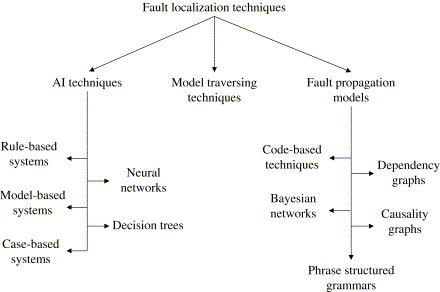
\includegraphics[width=0.5\textwidth]{Fig2}
\end{figure}

This paper presents the background research that has been done before paper 1 in section 2 - 4 and in section 5 presents the paper 1 \cite{pclee:07}.

\section{Expert Systems techniques}
Most widely used technique in the field of fault localization and diagnosis are expert systems as they try to mimic the actions of human expert. 
Most expert systems use rule based system as their inference engine. \cite{Peng:97},\cite{Liu:99} and \cite{Nygate:95} are examples of expert systems.

The expert systems developed differ in the knowledge they use. Rule based fault localization solely depend on the 
structure of the knowledge base as rule definition language. In \cite{Lor:93}   the knowledge base is divided to reusable 
knowledge modeled as core knowledge and customized knowledge.  in  \cite{Liu:99} the rules are organized as composite events and 
an intervention of human expert is required to update the event base.  The rule based systems can act as a powerful tool to eliminate 
least likely hypothesis. Although the RBR paradigm is appropriate for problem-solving tasks that are confined and well-understood its limitations are.

\begin{itemize}
  \item an in-ability to learn from experience.
  \item Fan inability to deal with novel problems.
  \item the difxulty of updating the systems to keep up with rapidiy changing domains such as expanding heterogeneous network.
\end{itemize}

in Model bases expert systems like \cite{Nygate:95} conditions are ususally accosiated with rules which includes predicates referring to system model. 
These predicates test the syetem for existence of relationship among system component. \cite{Nygate:95} 
uses correlation tree skeletons describing cause and effect relation ships between event. regardless of what expert system is being used localization process is 
always driven by inference engine and correaltion rules between events. 

\cite{Lewis:93} and \cite{Gardner:96} are examples of Case-based reasoning systems. The goals of CBR systems are (i) to learn from experience, (ii) to 
offer solutions to novel problems based on past experience, and (iii) to avoid expensive maintenance. The basic idea of CBR is to recall, adapt, and 
execute episodes of former problem-solving in an attempt to deal with a current problem. Former episodes of problem-solving are represented as cases in a case 
library. When confronted with a new problem, a CBR system retrieves a similar case and tries to adapt the case in an attempt to solve the outstanding problem. 
The disadvantages of such a system is the time complexity in retrieving a case that is the closest match to the event and the close tailoring of the application 
to the domain.

In addition to the above mentioned techniques there are other notable techniques are neural networks based approaches \cite{Gardner:97} \cite{Gardner:98} and 
decision tree based approaches \cite{Rodosek:98}. Neural networks have parallel computing architecture and are very fast avoiding bottlenecks which 
commonly arises from serial processing. But the main disadvantage is that the learning process requires intesive training  and in communication networks 
where all the alarms signatures are not readily available for pattern recognition.

Decision tree aproaches are simple and allows expressive representation of expert knowledge howeever they are limited by the dependencies sepcific 
applications nad degraded accuracy in noisy scenarios \cite{Russell:96} \cite{Koller:10}.

\section{Model traversing techniques}
\cite{Katker:96}, \cite{Katker:971}, \cite{Katker:97} and \cite{Gruschke:98} are all Model Traversing that use formal representation of communication 
system with clearly marked relationships across network entities. This technique identifies faults by traversing a model of entities starting form the entity whic reported an alarm and also involves a fault identification process to identify and locate faulty network entities.

The model representation used by this technique is object-oriented representation of the given system. It is based on the OSI management framework and uses GDMO (Guidelines for  Definition  of Managed Objects) with extensions to the MO to model dependencies and services between the entities. This approach can make automated testing possible which can test for various testing entities availability and quality of service standards. 

The event correlation in model traversing techniques is event driven as when an event occurs it is being mapped to the reported entity and the managed object representing that entity. For every event the search begins from the MO reporting the event and is searched recursively forllowing all relationship links between MO's using fault localization algorithms.  Fault localization algorithms used in this technique can be of various flavours.  models every event as singleton classes and merges them whenever they are traced to the same node. Typical proerties of such techniques involve 

\begin{itemize}
  \item Level at which a particular fault has occurred in the model.
  \item Event Type.
  \item Event severity.
  \item Event Origin - to identify if the event occurred is primary or secondary.
\end{itemize}

\begin{figure}[h!]
  \caption{Architecture of a model traversing technique prototype}
  \centering
    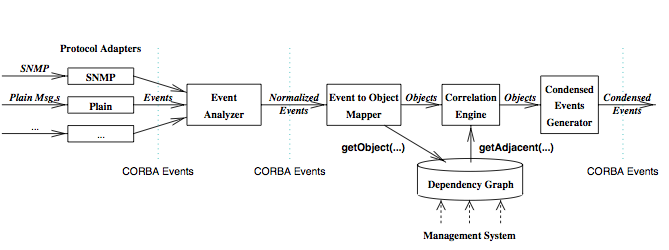
\includegraphics[width=0.5\textwidth]{Fig3}
\end{figure}

The MO's provide functions which lets the process test the entity for its operational status.  The root cause is found when the process stops at an entity and validates that it is a malfucntioning object and doesn't depend on any other object. In a multi layer model vertical search is performed first and then horizontal search in the next lower layer to check its peer at the end of search process votes are collected to identify the faulty elements and the device that recieves the most votes is declared faulty and a testing process kicks in to test the validity of the hypothesis. 

Model traversing techniques are pretty robust agianst network configuration changes and very useful in the scenario's where automated testing is a requirement and the depedency model is very natural as they are modeled as Trees or Graphs. 

The biggest drawback is the Fault Propagation Patterns and when there  fault is a logical combination of multiple devices and byzatine problems. It also incurs heavy testing costs. 

\section{Graph-theoretic techniques}
 
Grap theoretic techniques depend on gaphical model of a system called fault proppagation model(FPM). FPM represents fault and symptoms that occur in a system. 
The symptoms that are observed are mapped into nodes in the FPM and localization algorithms analyze the graph to infer the best explanation of the observed symptoms. 

These techniques require a knowlede of depedencies among the abstract and physical system components and how these failures in one component are related to 
other components. The success of the fault localiztion algorithm depends on the the accuracy of this a priori specification.

FPM's are genrally modeled as (i) Cuasaultiy graph is is a DAG whose nodes are events and edges represent the causality implications i.e cause effect relationships 
between events. They are carry probabilties to the nodes and edges implying the probability of a certain event to happen. 
Dependency Graph is a directed graph {\it{G=(O,D)}} where O represent a finite set of nodes and D are the depedency edges between Objects. 
The directed edge (o$_{i}$,o$_{j}$) $\in$ D represents that when o$_{i}$ fails o$_{j}$ fails or emits some kind of error. 
The edges are also labeled with conditional probabilities. Figure 4 represents such a depedency graph.

\begin{figure}[h!]
  \caption{A Network example along with the dependecy graph \cite{Katzela:95}}
  \centering
    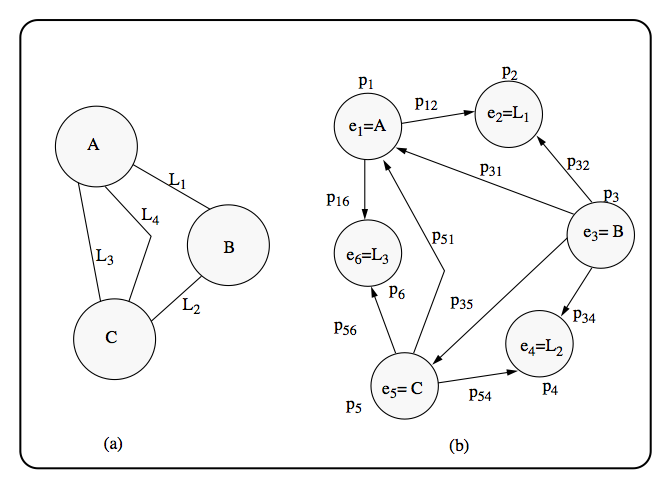
\includegraphics[width=0.5\textwidth]{Fig4}
\end{figure}

A lot of approaches using dependency graph, a critical assumption involves that an entity may fail in only one way. If that is the case the causal graph and dependecy graph would be the same.  In the case of multiple failures associated to a single entity they can be divided into sets such as {\it{complete failure, abnormal transmission delay, high packet loss, etc.}}. The dependecy graph in this case would have multiple edges between failure modes and the Object(entity). Sethi et all in \cite{Sethi:02}, \cite{Sethi:041}, \cite{Sethi:04} have modeled using multiple failure modes principle. 

A fault localalization algorithm, based on the provided FPM generally returns a number of hypothesis that best explain the observed symptoms. The problem of finding best explanation of the recieved alarms is {\it{NP-hard}} problem and proved in \cite{Katzela:95} by reducing the given problem to a Min Set-Cover problem.

\subsection{Divide and conquer algorithm}
The divide and conquer algorith uses a FPM assuming that one type of failure is allowed per object. It is a window based technique i.e gathers all the faults in a time window and analyzes them. 

System model is a directed graph G = ( E ,D) called the dependencygraph, where E is a finite nonempty set of active terminal objects e$_i$, and a directed edge (e$_i$, e$_j$) $\in$ D denotes the fact that a fault in e$_i$ has a side effect on e$_j$ i.e., e$_j$ is dependent on e$_i$.
Each vertex e$_i$ is assigned a weight p$_i$ that is the probability that the object e$_i$ fails independently of the state (failed or not failed) of any other active terminal object that is dependent on it. Each directed edge ( e$_j$,e$_i$) is assigned a weight p$_{ji}$ which represents the strength of dependency between the entities it connects. Specifically, p$_{ji}$ , is the conditional probability p$_{ji}$ = P(e$_j$ fails\textbar e$_i$ fails) that entity e$_j$, fails as a result of the failure of entity e$_i$. In addition, the weight of a directed path is defined as the product of all the weights of the edges that compose the path. Finally, the strength of dependency p$_{kl}$ between two non-adjacent vertices e$_k$ and e$_l$, is defined as the maximum of the weights of all directed paths from e$_k$ to e$_l$.

Let D(a$_i$) for every a$_i$ alarm be the domain of alarms that defines as the set of objects that might have caused the alarm.  The domain of an alarm calculation is a variation of single source problem that finds the min cost paths from a source vertex to all other graphs and the nodes are chosen such that the cost of path e$_i$ to e$_j$ is subject to restriction that we include only the minimum cost paths with cost $\leq$ log(W) where W is a parameter.

The outline of the algorithm run has been given below.

\begin{itemize}
  \item Start with the set S of objects associated with the alarm cluster.
  \item Find the partitioning of the set S resulting in two disjoint sets so in each set the objects exhibit the maximum mutual dependency, i.e., for every object e$_i$ and e$_j$, that belongs to the same set and e$_k$ that does not belong to the set, the dependency weight p$_{ij}$is greater than the dependency weights p$_{ik}$, p$_{ki}$, p$_{jk}$, p$_{kj}$.
  \item Of the two sets, select the one that explains all the received alarms and has the maximum probability that at least one of the entities in the set is a fault. If there is no such set then find the subset of alarms that each set explains and select both.
  \item Apply the previous two steps of the algorithm recursively to the selected sets until the resulting sets of the current partitioning are singletons.
\end{itemize}

By partitioning with the maximum mutual dependency criterion we group together objects that are highly dependent on each other and when the result of partitionining, both the sets are capable of explaingin all the alarms then we select one set that has higher probability of having one of them at fault. 

When determining atleast on memeber of the subset is faulty it is calcualted using. 

P(S) = ${\underset{\forall i:e_i \in S}{\sum}}[p_i + \underset{\forall j:e_j \in S , j \neq i}{\sum} p_{ij}.p_j]$


\begin{figure}[h!]
  \caption{Divide and Conquer algorithm \cite{Katzela:95}}
  \centering
    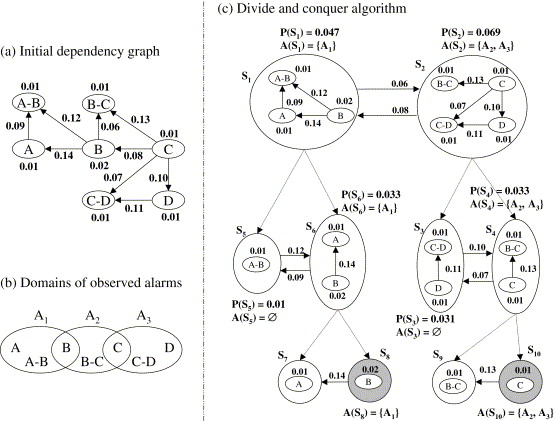
\includegraphics[width=0.5\textwidth]{Fig5}
\end{figure}

In algorithm runs in two phases where in the first phase algorithm finds the maximum mutual partitionings of the entities in the set S. The result of Phase I is a hierarchical clustering of the entities in the set S. In the Phase II a fault localization algorithm is recursively invoked to find the subsets that are supposed to be used. The first subcluster contains all alarms that may be explained using the subset with the higher probability that one of its members was a primary source of a failure. The second subcluster contains the remaining alarms from the original alarm cluster. Its domain is the other of the two subsets. The recursive procedure is then invoked twice, taking the two subclusters and their respective domains as parameters. The recursion continues until the input alarm cluster domain is a singleton. 

The algorithm mentioned above gives the explanation of the observed alarms but may not prouce the best output as it is a approximation algorithm based on maximum mutual dependency heuristic. The runtime complexity of the algorithm is O(N$^{3}$) and the partitioning phase runtime is O(logN). The drawback of the algorithm is it cannot handle the lost or spurious alarms and is a time window based determinsitic algorithm.

\subsection{Bayesian Reasoning approach}
Bayesian network or probabilistic graphical model represents a set of random varaibles and their conditional dependencies using a directed acyclic graph. In the context of fault localization the random variables represent the state of network entities and the occurrence of network events. 

\begin{figure}[h!]
  \caption{A example bayesian network}
  \centering
    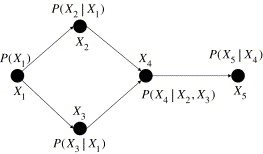
\includegraphics[width=0.5\textwidth]{Fig6}
\end{figure}

Belief networks are used to make four basic queries given evidence set e: belief assessment, most probable explanation, maximum a posteriori hypothesis, and maximum expected utililty \cite{Pearl:98}

\cite{Cynthia:97}, \cite{Sethi:02}, \cite{Sethi:041} and \cite{Sethi:04} all the papers try to model the FPM as a bayesian network using a layered fault model apparoach and in general fault component models are divided into services, protocols and functions. The recursive dependencies between services, protocols and functions constitue a dependenct graph. Uncertainty about dependencies between communication system entities is represented by assigning probabilities to the links and/or nodes in the dependency or causality graph. 

The queries for belief assesment and most probable explanation are of particular interest in the approaches mentioned above. The belief assesment task is to compute $bel(V_i=v_i) = P(V_i=v_i|e)$. given an evidence e, {\it bel}  gives the certainity of an event happening under the evidence. The most probable explanation task is to find an assignment that best explains the observed evidence e, i.e.,  \\
$P(A_{max}) = max_A \underset{i=1}{\overset{n}{\pi}} P(V_i=v_i^A | Par(V_i)^A)$ \cite{Pearl:98}. \\
It is known that the above tasks are NP-{\it hard} in the regular belief networks. A belief updating algorithm, polynomial with respect to $|$V$|$, is available for {\it polytrees}, i.e., directed graphs without undirected cycles. The exact calculation of the best explanatory hypothesis requires a number of steps that is exponential with respect to the number of graph nodes. One of the most popular exact algorithms bucket elimination is used as a reference algorithm against {\it iterative belief updating} algorithm and {\it iterative MPE query} algorithm.

\begin{figure}[h!]
  \caption{Bayesian Network message passing algorithm example}
  \centering
    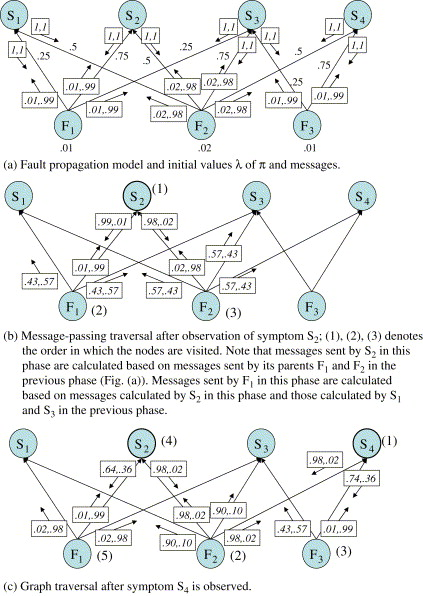
\includegraphics[width=0.5\textwidth]{Fig7}
\end{figure}

The algorithms  utilizes a message passing schema in which BN nodes exchange messages that encode certain conditional probabilities. The message that node X sends to its parent V$_j$ for every valid V$_j$'s value v$_j$ is denoted by ${\lambda}_X(v_j)$. The message that node X sends to its child U$_i$ for every valid value of X, x, is denoted by ${\pi}_{U_i}(x)$. Messages ${\lambda}_X(v_j)$ and ${\pi}_{U_i}(x)$ are calculated by node X based on messages it receives from its neighbors using the following equations (where $\beta$ is any constant and $\alpha$ is a normalizing constant)
\\
based on messages the {\it bel(x)={$\alpha$}{$\lambda$}(x){$\pi$}(x)}.

The alogirthm proceeds in an event driven manner when a symptom is observed and applying a message passing iteration traversing the graph based on an order. Figure 7 shows an example bayesian network with fault nodes F$_1$, F$_2$, F$_3$. Once the algorithm ends every node is assigned a belief probability, the probability of its existence given the symptoms. The final hypothesis is chosen using the following heuristic: (1) a most-likely fault is chosen and placed in the final hypothesis, (2) the chosen fault node is considered a part of evidence, and (4) one iteration of message passing starting from the chosen fault node is performed. Steps (1)–(3) are repeated as long as (1) the posterior distribution contains fault nodes whose probability is greater than 0.5, and (2) unexplained negative symptoms remain. An inherent property of the adapted algorithm is the capability to isolate multiple simultaneous faults even if their symptoms overlap. 

However one limitation to the modeling of the domain as bayesian network is the model has to adopt canonical models used in the literature mentioned above like noisy-OR gates, AND gates to limit the algorithm runtime to polynomial time. The comparision of different algorithms in bayesian networks is mentioned in the table 1 below.

\begin{center}
\begin{table*}[ht]
{\small
\hfill{}
    \begin{tabular}{ | c | c | c | c |}
    \hline
    Algorithm & Bucket Elimination & Iterative Belief Updating & Iterative MPE \\ \hline
    Theoretical Bound & $n^2$exp(n) & $n^5$ & $n^6$ \\ \hline
    Detection Rate & 96-100\% & 93-98\% & 95-100\% \\ \hline
    False Positive Rate & 0-4\% & 2-5\% & 0-8\% \\ \hline
    Max Network Size & 10 & 50 & 25 \\ \hline
    Algorithm iterative? & no & yes & yes \\
    \hline
    \end{tabular}}
\hfill{}
\caption{Comparision of algorithms}
\label{tb:tablename}
\end{table*}
\end{center}

\cite{Kandula:05} Shrink a tool for failrue diagnosis in IP Networks. Shrink outputs the most likely explanation for the network's faulty state –i.e., the collection of SRLGs whose failure is most likely given the IP link status. Shrink works on three modules (1) building the bayesian model (2) augemnting the model with guess edges (3) inferring the most likely explanation.

\begin{figure}[h!]
  \caption{Shrink system setup}
  \centering
    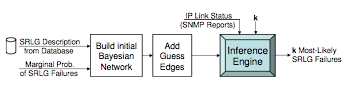
\includegraphics[width=0.5\textwidth]{Fig8}
\end{figure}

\begin{figure}[h!]
  \caption{Shrink's network model}
  \centering
    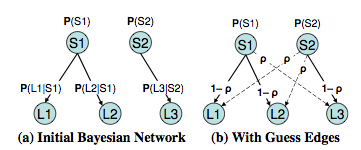
\includegraphics[width=0.5\textwidth]{Fig9}
\end{figure}

if $E_k$ denotes the event that at most k SRLGs failed within any hour, there are exactly k combinations of n possible SRLG assignmentsthat satisfy $E_k$. Given the observed link status, shrink algorithm greedily picks the most likely SRLG assignment in $E_k$; i.e., it picks $(S_1,.....,Sn)$ $\in$ $\{0,1\}^n$ such that: \\
$arg \underset{S_1,....,S_n}{max} P(S_1,.....,S_n|L_1,....L_n)$ subject to number of \{$S_i$=1\} $\leq$ k \\
There are fewer than $n^k$ value assignments in $E_k$, and for each assignment $P(S_1,...,S_n|L_1,...,L_m)$ can be computed in O(m + n) time, where m is the number of IP links and n is the number of SRLGs. So, Shrink’s running time is O($n^k$ ∗(m+n)). k=3 is a valid case for a wide range of ISP network sizes and SRLG failure probabilities and when k$\geq$3 the hypothesis performance is exponential. 

\subsection{Misc approaches}

There are several other approaches to fault localization like codebook approach which uses hamming distances to find the fault and also context free grammer which allows xpressions to be built from subexpressions, may be effectively used to represent a hierarchically organized communication system. However these are not discussed in this papaer due to the poor applicability to the real world systems and poor performance of these approaches. \cite{Calo:95}, \cite{Kliger:95}, \cite{Yemini:1996} are papers that discuss about these techiniques.

\section{Paper 1: Toward Optimal Network Fault Correction in Externally Managed Overlay Networks}
\cite{pclee:07} Paper 1 is an end-to-end approach of inferring probabilistic data-forwarding failures in an externally managed overlay network, where overlay nodes are independently operated by various administrative domains. The optimization goal is to minimize the expected cost of correcting (i.e., diagnosing and repairing) all faulty overlay nodes that cannot properly deliver data. Instead of first checking the most likely faulty nodes as in conventional fault localization problems it chooses a {\it candidate node} proceed based on a potential heuristic function and is bound to infer correctly atleast 95\% of the time.

\cite{Katzela:95}, \cite{Sethi:04} and \cite{Kandula:05} state of the art techniques that diagnose (i.e detect and localize) the components that are root causes of the network faults, however they do not focus on the {\it network fault correction} that is not only diagnosis but also considering the repair and checking costs. \cite{pclee:07} conveniently outperforms all of them and tries to derive a strategy for efficient network fault correction at minimum cost. 

Another set of research papers focus purely on the failure detection of network faults \cite{Zhuang:05}, \cite{Mizrak:05} and \cite{Avramopoulos:04} uses distributed techniques and all networks nodes to collaboratively achieve the fault detection. \cite{Avramopoulos:04} uses inspection on packets from previous hop and reports when founded corruption. The problem with this approach is that an inspection logic or monitoring points have to be setup across the network and incurs heavy costs and different administration domains prove to be obstacle in the above cases too. 

Paper1 considers and end-end inference approach using end-end measurements, infers components that are faulty in forwarding data. This applies perfectly to the scenario like CAN\cite{Ratnasamy:01} and CHORD\cite{Stoica:01} where each overlay node builds a routing tree with itself as a root and in this setting every root to leaf path is monitored to find faulty path and anamolous behaviours on the path. One anamoulous behaviour could be number of correct packets bot being delivered in a fixed time period, such a validation could prove to be very important in QOS factor.  The authors are particular interested in diagonize and repairing faulty nodes in overlay networks like RON\cite{Andersen:01}, SON\cite{Duan:03} and SOS\cite{Misra:04}. The proposed fault correction mechanism suits well to this type of  networks. 

\subsection{Problem Formulation}
\cite{pclee:07} considers a logical tree as T=$(N,\{{p_i}\},\{{c_i}\}),$ where N is the set of overlay nodes, $p_i$ is the failure probability of node i$\in$N, and $c_i$ is the checking cost of deciding if node i$\in$N is faulty. Overlay set node N provides a topology information and sequence of nodes. The construction of failure probabilities and cost probabilities depend on Failure model and Cost model.

{\bf Failure Model} focus on the nodes that cannot forward data or fails to comply with a QOS because of which packets get dropped or fails to get delivered. Focus mainly stands on fail-stop failues like power outages, full transmission queues, hardware errors and route misconfigurations. The failure probabilities are calculated using statistical measurements of reliability indexes of node elements(vulnerability modelling).  Authors also performed analysis of the  mechanism under inaacurate probabilities and is provide in the results section of this paper. Important consideration to be made is that failure probabilities of nodes are independent of each other. 

{\bf Cost Model} provides the checking costs using personnel hours, wages and time effort that goes into debugging the problem or even the cost of the equipment. Important cirteria to be noted in the cost model the repair costs are not conisdered as eventually every fault has to be repaired. $p_i$ and $c_i$ can be any values between [0,1] and [0,$\infty$].

Each node in a logical tree T is classified as fault or non-faulty. and definitions are being made on each root to leaf path that exhibits an anamalous behaviour. Since an end-to-end inference mechanism is being made we only know that something is wrong with the path rather than which node is at fault. Each node in T is referred to as {\it bad} if it is faulty and {\it good} if it is non-faulty and a path in T is bad if it has atleast one {\it bad} node. An important consideration is that the node behaviour remains the same across all the paths as only fail-stop considerations are being made. 

Given a logical tree T we can infer the good path and bad paths by end to end inference mechanism, for example root can send a probe and collect all measurement results. We now create a bad Tree by pruning of all the good paths form the logical tree and also call it T with abuse of notation. Bad tree now becoms input to the inference algorithm which determines which set of nodes to be corrected(checked and repaired).

The optimization goal of this paper is to minimize the expected cost of correcting all faulty nodes in a given tree. repairing cost is not considered as eventually all the nodes have to be repaired and any strategy that is employed will eventually correct all the nodes. Here we focus only on the sequential case as checking the nodes in parallel doesnt improve the total expected checking cost so the inference algorithm only return one single node that is supposed to be the best node to check first. The best node is the first node that is from a diagnostic sequence {\it S} = $\{l_1,l_2,....,l_N\}$ and gives us {\it N!} diagnositic sequences.

When a particular node {\it $l_i$} lies on a bad path we do no know whether it is a good node or a bad node but if it is on a good node we know for sure it is a good node. {\it $l_i$}  gets {\it checked or skipped} based on the examination of the node. Thus we can summarize the total cost of checking a tree {\it T} is given by  \\
$\underset{i=1}{\overset{|N|}{\sum}} c_{l_i} Pr(node\ l_i\ is\ checked\ | \ nodes\ l_1,...,l_{i-1}\ known\ to\ be\ good)$ \\
So the best node would be the first node in the diagnosis sequence and the inference works on the current topolgy to indetify this node and when the node is corrected the revised topology is fed into the inference algorithm to output the next node. The total complexity of calculating the expected cost of a diganosis sequence is O($n^3$) and since there are n! differenct sequences, the brute force approach has a complexity of O($n^3$n!). The complexity and the way to calculate the total cost for the diagnostic sequence is mentioned in Appendix A of \cite{pclee:07}. In the interest of space and lenth only the highights are being mentioned here.

{\bf Conditional Failure Probabilties}: the nodes in T by 1 to $|$N$|$ in breadth- first-search order. $T_i$ is the subtree rooted at node i. $C_i$ is the set such that k$\in$$C_i$ if node k is a   child node of {\it i}. thus conditional failure probability is given by bayesian probability rule where Pr($X_i$) is the independent failure probability of a node, and Pr($T_1$) is the probability of the tree is bad at root, $Pr(T_1|X_i)$ is the probability that a tree is a bad tree upon the event that a node is bad. \\
$Pr(X_i|T_1) = \frac{Pr(T_1|X_i)Pr(X_i)}{Pr(T_1)}$ by baye's rule.\\
where\\
$Pr(T_i) = p_i+(1-p_i) \underset{k{\in}C_i}{\pi}Pr(T_k) , \forall i \in [1,|N|]$\\
\\

\[
 Pr(T_i|X_j) =
  \begin{cases}
   Pr(T_i) & \text{if } i > j \\
   1       & \text{if } i=j \\
   p_i+(1-p_i)  \underset{k{\in}C_i}{\pi} Pr(T_k|X_j)  & \text{if } i<j
  \end{cases}
\] \\

The idea here is that a subtree $T_i$ is bad if either the node itself is bad or node {\it i} is good and the subtree rooted at {\it i} is bad. Using dyanmic programming the above equation can be computed in O($N^2$) which is the conditional failure probabitlity of a node. 

{\bf Expected Cost of  a Diagnosis Sequence}: Let ${T_{l_i}}^D$ be the event that the subtree rooted at node ${l_i}$ is a bad tree after nodes ${{l_1},...,{l_{i-1}}}$ have been examined (i.e., checked or skipped). Let ${A_{l_i}}^D$ be the event that every ancestor j of node ${l_i}$, such that j $\in\{l_{i+1},...,l_{|N|}\}$ (i.e., node j is examined after node ${l_i}$), is a good node. Since every node is examined in a sequential way in the diagnosis sequence, when $l_i$ is examined, nodes $l_1,....,l_{i-1}$ have been examined and they are good. Thus, \\
$Pr({T_{l_i}}^D) = Pr(T_{l_i}|p_{l_1}= ... = p_{l_{i-1}} = 0)$, and \\
$Pr({A_{l_i}}^D) = Pr(A_{l_i}|p_{l_1}= ... = p_{l_{i-1}} = 0)$ \\
Where $T_{l_i}$ is the event that the subtree rooted at node $l_i$ is bad, and $A_{l_i}$ is the event that all ancestors of node $l_i$ are good. If the subtree rooted at node $l_i$ remains a bad tree or at least one of the ancestors of node $l_i$ is a bad node, then node $l_i$ still lies on bad path and needs to be checked. Thus, \\
$ Pr(node\ l_i\ is\ checked| T, nodes\ l_1,...,l_{i-1} known\ to\ be\ good)$ \\
$=Pr({T_{l_i}}^D \cup \neg{{A_{l_i}}^D} | T)$\\
Thus the expected cost of S given that T is a bad tree is: \\
\center$ \underset{i=1}{\overset{n}{\sum}} c_{l_i} Pr({T_{l_i}}^D \cup \neg{{A_{l_i}}^D} | T)$\\
Brute force algorithm which inspects all the sequences is given in figure 10. This algorithm makes a good reference for comapring against the heuristic based ones.

\begin{figure}[h!]
  \caption{Bruce Force Algorithm}
  \centering
    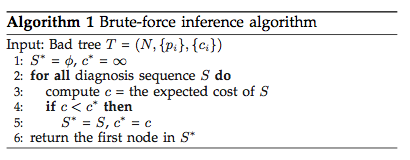
\includegraphics[width=0.5\textwidth]{Fig10}
\end{figure}

\subsection{Naive Heuristics for Inference Algorithm}
Intuitively the best node returned by the inference algorithm can be either based on the highest conditional failure probabiltiy or checking cost.  The authors provided a simple counter example in which neither the selection of node based on conditional failure probability nor the one selected based on checking cost gave the optimal solution. The three heuristics authors chose naively are (1) {\it Naive_Prob} (2) {\it Naive_Cost} (3) {\it Naive_Prob_Cost} . Based on the experimental setup where a 200 bad trees are tested with the three heuristic mentioned above with varying probabiltiy and cost distributions. Depending on the distributions of $p_i$ and $c_i$, the proportion of instances where the best choice is made can be as low as 10\% for Naive-Prob and Naive-Cost  and less than 55\% for Naive-Prob-Cost.
\begin{figure}[h!]
  \caption{Naive-Prob, Naive-Cost, and Naive-Prob-Cost performance}
  \centering
    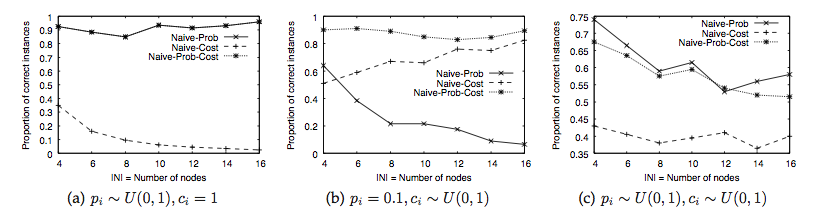
\includegraphics[width=0.5\textwidth]{Fig11}
\end{figure}

\subsection{Candidate Node}
The authors show that instead of selecting a node to test based on naive choices we should select a {\it candidate node} based on the maximization of a {\it potential function}. Let $A_i$ be the event that the ancestors of node {\it i} are all good. If node {\it r} is the root node, then we let $A_r$ be always true and $Pr(A_r) = 1$. The potential of a candidate node is calculated using the formula. \\
                        \center $\phi({\it i,T)} = \frac{Pr(T|X_i,A_i)p_i}{c_i(1-p_i)}$
\appendix
%\bibliographystyle{abbrv}
%\bibliography{sigproc}


%
% sample.tex
% $Id: sample.tex,v 1.1 2006/03/18 00:21:36 johnh Exp johnh $
%


% The default of sigplan-proc-varsize is 9pt, indented paragraphs (acm style)
% For Sensys or other 10pt conference, use the 10pt option
%\documentclass{sigplan-proc-varsize}
% options:
%\documentclass[9pt]{sigplan-proc-varsize}
\documentclass[10pt]{sigplan-proc-varsize}
%\documentclass[noindentedparagraphs]{sigplan-proc-varsize}



% % hack to avoid the ugly ACM paragraph definition
% % => can't leave blank line after this
% (remove comment for this hack)
% \renewcommand{\paragraph}[1]{\vskip 6pt\noindent\textbf{#1 }}
\usepackage{amsmath}
\usepackage{graphicx}
\usepackage{url}
\usepackage{underscore}


\numberofauthors{1}


\author{
%
% The command \alignauthor (no curly braces needed) should
% precede each author name, affiliation/snail-mail address and
% e-mail address. Additionally, tag each line of
% affiliation/address with \affaddr, and tag the
%% e-mail address with \email.
\alignauthor Vijay Akkineni \\
        \affaddr{Department of Computer Science and Engineering}\\
        \affaddr{Georgia State University}\\
       \email{vakkineni1@student.gsu.edu}
}

\title{Fault localization in Communication Networks}

%\conferenceinfo{Phd Qualifiers'13,} {September 6, 2013, Atlanta, United States.}
%\CopyrightYear{2013}

\begin{document}

\maketitle

\begin{abstract}
This paper is about fault localization techniques in communication networks worked for Phd qualifiers examination. 
Fault Localization is an important aspect of network fault management and is a process of deducing the source of a failure from the set of observed indicatations. 
It has been an important research area in the field of networking both communication networks and wireless sensor networks.
As commuication networks grow in size and complexity it has been imposing new set of requirements on fault localization. 
Despite the amount of research done in this field we can still argue that it is an area of open for research. 
The paper essentially disucsses the work that has been done in this field in the pas few years with emphasis on the both the papers given for the examination.
\end{abstract}

% A category with the (minimum) three required fields
\category{H.4}{Communication Networks, Sensor Network Applications}{Miscellaneous}

\keywords{Fault Localization, Communication Networks, Root Cause Analysis, Causal Inference}

\section{Introduction}
  \label{sec:intro}

Fault diagnosis is an important part of networking. Faults are unavoidable in communication systems but their quick detection and isolation and repair is critical 
for the robustness, reliability and health of the system. When the networks get large and cumbersome automatic fault diagnosis and fault management is a crucial aspect.

A basic taxonomy in this field is mentioned below.

Event, defined as an exceptional condition occurring in the operation of hardware or software of a managed network, is a central concept pertaining to fault diagnosis.

Faults (also referred to as problems or root causes) constitute a class of network events that can cause other events but are not themselves caused by other 
events. Faults may be classified as: (1) permanent, (2) intermittent, and (3) transient. A permanent fault exists in a network until a repair action is taken.
Intermittent faults occur on a discontinuous and periodic basis causing a degradation of service for short periods of time.
However, frequently re-occurring intermittent faults significantly jeopardize service performance. 
Transient faults cause a temporary and minor degradation of service.

Error(Failure) is defined as a discrepancy between a computed, observed, or measured value or condition and a true, specified, or theoretically correct value or condition. 
Error is a consequence of a fault. Faults may or may not cause one or more errors. 
Errors may cause deviation of a delivered service from the specified service, which is visible to the outside world. 
Errors do not need to be directly corrected, and in many cases they are not visible externally. 
However, an error in a network device or software may cause a malfunctioning of dependent network devices or software. 
Thus, errors may propagate within the network causing failures of faultless hardware or software.

Symptoms are external manifestations of failures. They are observed as alarms—notifications of a potential failure. 
These notifications may originate from management agents via management protocol messages (SNMP trap and CMIP EVENT-REPORT), 
from management systems that monitor the network status, e.g., using command ping, system log-files or character streams sent by external equipments.

Figure 1 shows the concepts described above in an end to end perspective.

The process of fault diagnosis usually involves three steps as cited in \cite{KatzelaThesis:1996}:

\begin{itemize}
  \item Fault detection, a process of capturing on-line indications of network disorder provided by malfunctioning devices or fault detection agents in the 
  form of alarms.
  \item Fault localization (also referred to as fault isolation, alarm/event correlation, and root cause analysis) is a set of observed fault indications is analyzed to 
  find an explanation of the alarms.
  \item Testing is a process that, given a number of possible explanations, determines the actual faults.
  \item Fault Correction, by which we mean not only to diagnose, but
also to repair all faulty components within a network (This includes the testing component).
\end{itemize}

\begin{figure}[h!]
  \caption{Distinction between fault, error and symptom}
  \centering
    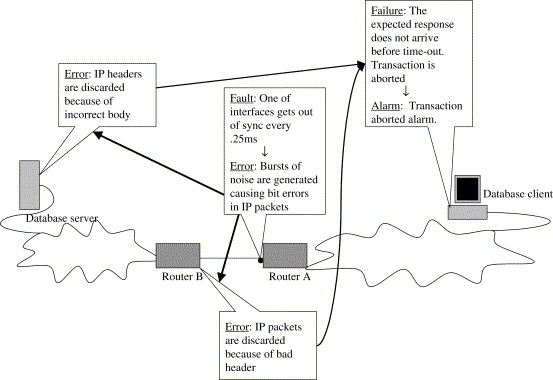
\includegraphics[width=0.5\textwidth]{Fig1}
\end{figure}

The difficulty in the fault localization process arise from the ambiguity of the observed set of alarms as same alarm can be generated from multiple different faults 
and multiple alarms can correlate back to the same fault. The incompleteness of the alarm stems from the fact that the alarm doesn't have all the information or 
there is a loss of alarm. Inconsistency among the observed alarms results from device perception of the fault is different form device to device.  

A set of alarms generated by a fault may depend on many factors such as dependencies among network devices, current configurations, services in use since 
fault occurrence, presence of other faults, values of other network parameters, etc. Due to this non-determinism the system knowledge may be subject to inaccuracy 
and inconsistency. Fault evidence may also be inaccurate because of spurious alarms, which are generated by transient problems or as a result of overly sensitive 
fault detection mechanisms. When spurious symptoms may occur, the management system may not be sure which observed alarms should be taken into account in the fault 
localization process. Event management systems should identify and eliminate multiple simultaneous related or unrelated root causes. 

In large networks distributed fault localization process should be performed in distributed fashion. Many researches \cite{Katzela:1995} and \cite{Yemini:1996} have 
concluded that distributed fault localization using a set of event management nodes is a better approach than centralized process. The complexity arised from the nature 
of error propogation, they propogate either horizontally to the peers or vertically from bottom layer to upper layers or afecting higher level services. The errors also
propogate from one management domain to a different management domain making the process even difficult. Therefore the distribution of complexity to distributed fault 
localization processes and inferring form the collective process makes the process computationally feasible and efficient. 

An alarm can insinuate different type of faults that occurred in different communication devices where in fault localization process may not comeup with a 
definitive answer. Few approaches that will be discussed in this paper combine fault localization with testing and fault ocrrection process to validate the hypothesis. 
Therefore there should be some kind of optimality measure or confidence measure that should be employed in measuring the hypothesis that the localization process 
came up with and it could include the lowest cost or min failure probability or some heuristic function which optimizes the process of validating the hypothesis.

Numerous works have been proposed on fault localization process. The techniques are dervice from different areas of artificial intelligence, graph theory, 
neural networks, automata theory and many other approaches. Figure 2 broadly classifies the exisiting solutions. The two papers provided for the exam falls into the 
category of end to end testing scenarios and proababilistic reasoning and derive their roots from bayesian network analysis. 

\begin{figure}[h!]
  \caption{Classification of fault localization techniques}
  \centering
    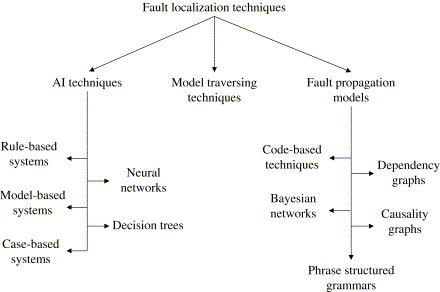
\includegraphics[width=0.5\textwidth]{Fig2}
\end{figure}

This paper presents the background research that has been done before paper 1 in section 2 - 4 and in section 5 presents the paper 1 \cite{pclee:07}.

\section{Expert Systems techniques}
Most widely used technique in the field of fault localization and diagnosis are expert systems as they try to mimic the actions of human expert. 
Most expert systems use rule based system as their inference engine. \cite{Peng:97},\cite{Liu:99} and \cite{Nygate:95} are examples of expert systems.

The expert systems developed differ in the knowledge they use. Rule based fault localization solely depend on the 
structure of the knowledge base as rule definition language. In \cite{Lor:93}   the knowledge base is divided to reusable 
knowledge modeled as core knowledge and customized knowledge.  in  \cite{Liu:99} the rules are organized as composite events and 
an intervention of human expert is required to update the event base.  The rule based systems can act as a powerful tool to eliminate 
least likely hypothesis. Although the RBR paradigm is appropriate for problem-solving tasks that are confined and well-understood its limitations are.

\begin{itemize}
  \item an in-ability to learn from experience.
  \item Fan inability to deal with novel problems.
  \item the difxulty of updating the systems to keep up with rapidiy changing domains such as expanding heterogeneous network.
\end{itemize}

in Model bases expert systems like \cite{Nygate:95} conditions are ususally accosiated with rules which includes predicates referring to system model. 
These predicates test the syetem for existence of relationship among system component. \cite{Nygate:95} 
uses correlation tree skeletons describing cause and effect relation ships between event. regardless of what expert system is being used localization process is 
always driven by inference engine and correaltion rules between events. 

\cite{Lewis:93} and \cite{Gardner:96} are examples of Case-based reasoning systems. The goals of CBR systems are (i) to learn from experience, (ii) to 
offer solutions to novel problems based on past experience, and (iii) to avoid expensive maintenance. The basic idea of CBR is to recall, adapt, and 
execute episodes of former problem-solving in an attempt to deal with a current problem. Former episodes of problem-solving are represented as cases in a case 
library. When confronted with a new problem, a CBR system retrieves a similar case and tries to adapt the case in an attempt to solve the outstanding problem. 
The disadvantages of such a system is the time complexity in retrieving a case that is the closest match to the event and the close tailoring of the application 
to the domain.

In addition to the above mentioned techniques there are other notable techniques are neural networks based approaches \cite{Gardner:97} \cite{Gardner:98} and 
decision tree based approaches \cite{Rodosek:98}. Neural networks have parallel computing architecture and are very fast avoiding bottlenecks which 
commonly arises from serial processing. But the main disadvantage is that the learning process requires intesive training  and in communication networks 
where all the alarms signatures are not readily available for pattern recognition.

Decision tree aproaches are simple and allows expressive representation of expert knowledge howeever they are limited by the dependencies sepcific 
applications nad degraded accuracy in noisy scenarios \cite{Russell:96} \cite{Koller:10}.

\section{Model traversing techniques}
\cite{Katker:96}, \cite{Katker:971}, \cite{Katker:97} and \cite{Gruschke:98} are all Model Traversing that use formal representation of communication 
system with clearly marked relationships across network entities. This technique identifies faults by traversing a model of entities starting form the entity whic reported an alarm and also involves a fault identification process to identify and locate faulty network entities.

The model representation used by this technique is object-oriented representation of the given system. It is based on the OSI management framework and uses GDMO (Guidelines for  Definition  of Managed Objects) with extensions to the MO to model dependencies and services between the entities. This approach can make automated testing possible which can test for various testing entities availability and quality of service standards. 

The event correlation in model traversing techniques is event driven as when an event occurs it is being mapped to the reported entity and the managed object representing that entity. For every event the search begins from the MO reporting the event and is searched recursively forllowing all relationship links between MO's using fault localization algorithms.  Fault localization algorithms used in this technique can be of various flavours.  models every event as singleton classes and merges them whenever they are traced to the same node. Typical proerties of such techniques involve 

\begin{itemize}
  \item Level at which a particular fault has occurred in the model.
  \item Event Type.
  \item Event severity.
  \item Event Origin - to identify if the event occurred is primary or secondary.
\end{itemize}

\begin{figure}[h!]
  \caption{Architecture of a model traversing technique prototype}
  \centering
    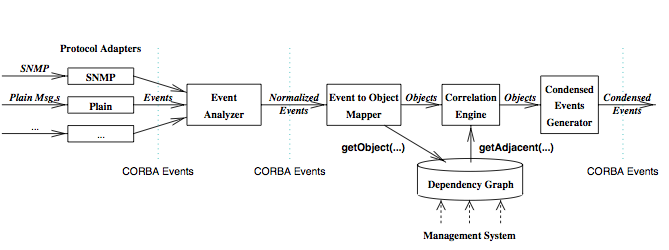
\includegraphics[width=0.5\textwidth]{Fig3}
\end{figure}

The MO's provide functions which lets the process test the entity for its operational status.  The root cause is found when the process stops at an entity and validates that it is a malfucntioning object and doesn't depend on any other object. In a multi layer model vertical search is performed first and then horizontal search in the next lower layer to check its peer at the end of search process votes are collected to identify the faulty elements and the device that recieves the most votes is declared faulty and a testing process kicks in to test the validity of the hypothesis. 

Model traversing techniques are pretty robust agianst network configuration changes and very useful in the scenario's where automated testing is a requirement and the depedency model is very natural as they are modeled as Trees or Graphs. 

The biggest drawback is the Fault Propagation Patterns and when there  fault is a logical combination of multiple devices and byzatine problems. It also incurs heavy testing costs. 

\section{Graph-theoretic techniques}
 
Grap theoretic techniques depend on gaphical model of a system called fault proppagation model(FPM). FPM represents fault and symptoms that occur in a system. 
The symptoms that are observed are mapped into nodes in the FPM and localization algorithms analyze the graph to infer the best explanation of the observed symptoms. 

These techniques require a knowlede of depedencies among the abstract and physical system components and how these failures in one component are related to 
other components. The success of the fault localiztion algorithm depends on the the accuracy of this a priori specification.

FPM's are genrally modeled as (i) Cuasaultiy graph is is a DAG whose nodes are events and edges represent the causality implications i.e cause effect relationships 
between events. They are carry probabilties to the nodes and edges implying the probability of a certain event to happen. 
Dependency Graph is a directed graph {\it{G=(O,D)}} where O represent a finite set of nodes and D are the depedency edges between Objects. 
The directed edge (o$_{i}$,o$_{j}$) $\in$ D represents that when o$_{i}$ fails o$_{j}$ fails or emits some kind of error. 
The edges are also labeled with conditional probabilities. Figure 4 represents such a depedency graph.

\begin{figure}[h!]
  \caption{A Network example along with the dependecy graph \cite{Katzela:95}}
  \centering
    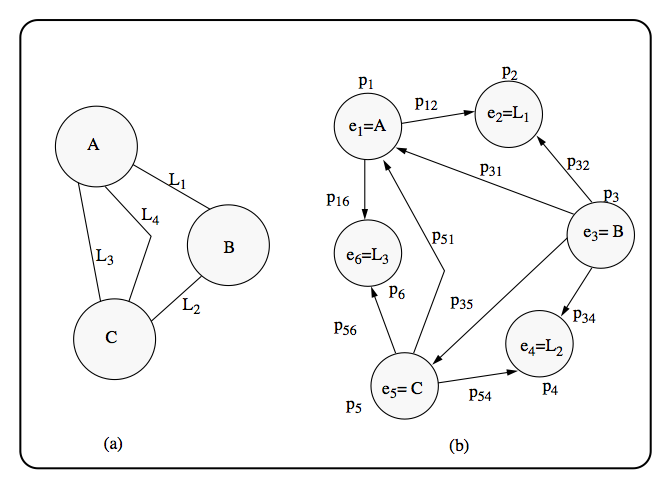
\includegraphics[width=0.5\textwidth]{Fig4}
\end{figure}

A lot of approaches using dependency graph, a critical assumption involves that an entity may fail in only one way. If that is the case the causal graph and dependecy graph would be the same.  In the case of multiple failures associated to a single entity they can be divided into sets such as {\it{complete failure, abnormal transmission delay, high packet loss, etc.}}. The dependecy graph in this case would have multiple edges between failure modes and the Object(entity). Sethi et all in \cite{Sethi:02}, \cite{Sethi:041}, \cite{Sethi:04} have modeled using multiple failure modes principle. 

A fault localalization algorithm, based on the provided FPM generally returns a number of hypothesis that best explain the observed symptoms. The problem of finding best explanation of the recieved alarms is {\it{NP-hard}} problem and proved in \cite{Katzela:95} by reducing the given problem to a Min Set-Cover problem.

\subsection{Divide and conquer algorithm}
The divide and conquer algorith uses a FPM assuming that one type of failure is allowed per object. It is a window based technique i.e gathers all the faults in a time window and analyzes them. 

System model is a directed graph G = ( E ,D) called the dependencygraph, where E is a finite nonempty set of active terminal objects e$_i$, and a directed edge (e$_i$, e$_j$) $\in$ D denotes the fact that a fault in e$_i$ has a side effect on e$_j$ i.e., e$_j$ is dependent on e$_i$.
Each vertex e$_i$ is assigned a weight p$_i$ that is the probability that the object e$_i$ fails independently of the state (failed or not failed) of any other active terminal object that is dependent on it. Each directed edge ( e$_j$,e$_i$) is assigned a weight p$_{ji}$ which represents the strength of dependency between the entities it connects. Specifically, p$_{ji}$ , is the conditional probability p$_{ji}$ = P(e$_j$ fails\textbar e$_i$ fails) that entity e$_j$, fails as a result of the failure of entity e$_i$. In addition, the weight of a directed path is defined as the product of all the weights of the edges that compose the path. Finally, the strength of dependency p$_{kl}$ between two non-adjacent vertices e$_k$ and e$_l$, is defined as the maximum of the weights of all directed paths from e$_k$ to e$_l$.

Let D(a$_i$) for every a$_i$ alarm be the domain of alarms that defines as the set of objects that might have caused the alarm.  The domain of an alarm calculation is a variation of single source problem that finds the min cost paths from a source vertex to all other graphs and the nodes are chosen such that the cost of path e$_i$ to e$_j$ is subject to restriction that we include only the minimum cost paths with cost $\leq$ log(W) where W is a parameter.

The outline of the algorithm run has been given below.

\begin{itemize}
  \item Start with the set S of objects associated with the alarm cluster.
  \item Find the partitioning of the set S resulting in two disjoint sets so in each set the objects exhibit the maximum mutual dependency, i.e., for every object e$_i$ and e$_j$, that belongs to the same set and e$_k$ that does not belong to the set, the dependency weight p$_{ij}$is greater than the dependency weights p$_{ik}$, p$_{ki}$, p$_{jk}$, p$_{kj}$.
  \item Of the two sets, select the one that explains all the received alarms and has the maximum probability that at least one of the entities in the set is a fault. If there is no such set then find the subset of alarms that each set explains and select both.
  \item Apply the previous two steps of the algorithm recursively to the selected sets until the resulting sets of the current partitioning are singletons.
\end{itemize}

By partitioning with the maximum mutual dependency criterion we group together objects that are highly dependent on each other and when the result of partitionining, both the sets are capable of explaingin all the alarms then we select one set that has higher probability of having one of them at fault. 

When determining atleast on memeber of the subset is faulty it is calcualted using. 

P(S) = ${\underset{\forall i:e_i \in S}{\sum}}[p_i + \underset{\forall j:e_j \in S , j \neq i}{\sum} p_{ij}.p_j]$


\begin{figure}[h!]
  \caption{Divide and Conquer algorithm \cite{Katzela:95}}
  \centering
    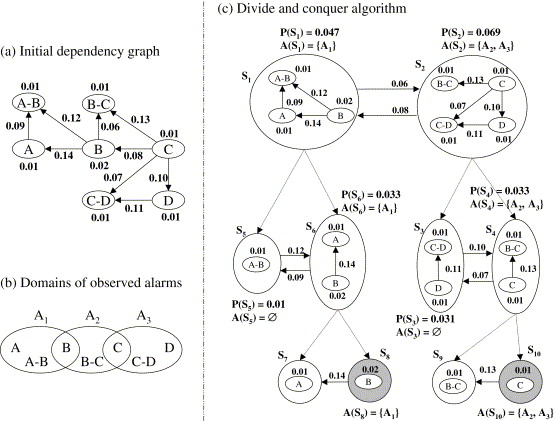
\includegraphics[width=0.5\textwidth]{Fig5}
\end{figure}

In algorithm runs in two phases where in the first phase algorithm finds the maximum mutual partitionings of the entities in the set S. The result of Phase I is a hierarchical clustering of the entities in the set S. In the Phase II a fault localization algorithm is recursively invoked to find the subsets that are supposed to be used. The first subcluster contains all alarms that may be explained using the subset with the higher probability that one of its members was a primary source of a failure. The second subcluster contains the remaining alarms from the original alarm cluster. Its domain is the other of the two subsets. The recursive procedure is then invoked twice, taking the two subclusters and their respective domains as parameters. The recursion continues until the input alarm cluster domain is a singleton. 

The algorithm mentioned above gives the explanation of the observed alarms but may not prouce the best output as it is a approximation algorithm based on maximum mutual dependency heuristic. The runtime complexity of the algorithm is O(N$^{3}$) and the partitioning phase runtime is O(logN). The drawback of the algorithm is it cannot handle the lost or spurious alarms and is a time window based determinsitic algorithm.

\subsection{Bayesian Reasoning approach}
Bayesian network or probabilistic graphical model represents a set of random varaibles and their conditional dependencies using a directed acyclic graph. In the context of fault localization the random variables represent the state of network entities and the occurrence of network events. 

\begin{figure}[h!]
  \caption{A example bayesian network}
  \centering
    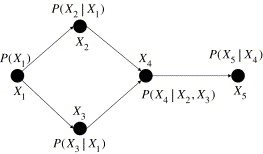
\includegraphics[width=0.5\textwidth]{Fig6}
\end{figure}

Belief networks are used to make four basic queries given evidence set e: belief assessment, most probable explanation, maximum a posteriori hypothesis, and maximum expected utililty \cite{Pearl:98}

\cite{Cynthia:97}, \cite{Sethi:02}, \cite{Sethi:041} and \cite{Sethi:04} all the papers try to model the FPM as a bayesian network using a layered fault model apparoach and in general fault component models are divided into services, protocols and functions. The recursive dependencies between services, protocols and functions constitue a dependenct graph. Uncertainty about dependencies between communication system entities is represented by assigning probabilities to the links and/or nodes in the dependency or causality graph. 

The queries for belief assesment and most probable explanation are of particular interest in the approaches mentioned above. The belief assesment task is to compute $bel(V_i=v_i) = P(V_i=v_i|e)$. given an evidence e, {\it bel}  gives the certainity of an event happening under the evidence. The most probable explanation task is to find an assignment that best explains the observed evidence e, i.e.,  \\
$P(A_{max}) = max_A \underset{i=1}{\overset{n}{\pi}} P(V_i=v_i^A | Par(V_i)^A)$ \cite{Pearl:98}. \\
It is known that the above tasks are NP-{\it hard} in the regular belief networks. A belief updating algorithm, polynomial with respect to $|$V$|$, is available for {\it polytrees}, i.e., directed graphs without undirected cycles. The exact calculation of the best explanatory hypothesis requires a number of steps that is exponential with respect to the number of graph nodes. One of the most popular exact algorithms bucket elimination is used as a reference algorithm against {\it iterative belief updating} algorithm and {\it iterative MPE query} algorithm.

\begin{figure}[h!]
  \caption{Bayesian Network message passing algorithm example}
  \centering
    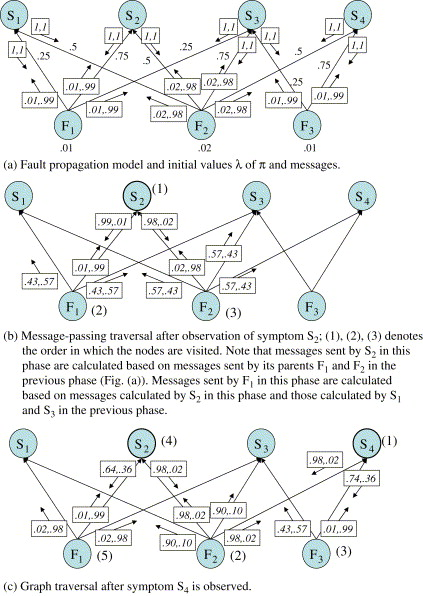
\includegraphics[width=0.5\textwidth]{Fig7}
\end{figure}

The algorithms  utilizes a message passing schema in which BN nodes exchange messages that encode certain conditional probabilities. The message that node X sends to its parent V$_j$ for every valid V$_j$'s value v$_j$ is denoted by ${\lambda}_X(v_j)$. The message that node X sends to its child U$_i$ for every valid value of X, x, is denoted by ${\pi}_{U_i}(x)$. Messages ${\lambda}_X(v_j)$ and ${\pi}_{U_i}(x)$ are calculated by node X based on messages it receives from its neighbors using the following equations (where $\beta$ is any constant and $\alpha$ is a normalizing constant)
\\
based on messages the {\it bel(x)={$\alpha$}{$\lambda$}(x){$\pi$}(x)}.

The alogirthm proceeds in an event driven manner when a symptom is observed and applying a message passing iteration traversing the graph based on an order. Figure 7 shows an example bayesian network with fault nodes F$_1$, F$_2$, F$_3$. Once the algorithm ends every node is assigned a belief probability, the probability of its existence given the symptoms. The final hypothesis is chosen using the following heuristic: (1) a most-likely fault is chosen and placed in the final hypothesis, (2) the chosen fault node is considered a part of evidence, and (4) one iteration of message passing starting from the chosen fault node is performed. Steps (1)–(3) are repeated as long as (1) the posterior distribution contains fault nodes whose probability is greater than 0.5, and (2) unexplained negative symptoms remain. An inherent property of the adapted algorithm is the capability to isolate multiple simultaneous faults even if their symptoms overlap. 

However one limitation to the modeling of the domain as bayesian network is the model has to adopt canonical models used in the literature mentioned above like noisy-OR gates, AND gates to limit the algorithm runtime to polynomial time. The comparision of different algorithms in bayesian networks is mentioned in the table 1 below.

\begin{center}
\begin{table*}[ht]
{\small
\hfill{}
    \begin{tabular}{ | c | c | c | c |}
    \hline
    Algorithm & Bucket Elimination & Iterative Belief Updating & Iterative MPE \\ \hline
    Theoretical Bound & $n^2$exp(n) & $n^5$ & $n^6$ \\ \hline
    Detection Rate & 96-100\% & 93-98\% & 95-100\% \\ \hline
    False Positive Rate & 0-4\% & 2-5\% & 0-8\% \\ \hline
    Max Network Size & 10 & 50 & 25 \\ \hline
    Algorithm iterative? & no & yes & yes \\
    \hline
    \end{tabular}}
\hfill{}
\caption{Comparision of algorithms}
\label{tb:tablename}
\end{table*}
\end{center}

\cite{Kandula:05} Shrink a tool for failrue diagnosis in IP Networks. Shrink outputs the most likely explanation for the network's faulty state –i.e., the collection of SRLGs whose failure is most likely given the IP link status. Shrink works on three modules (1) building the bayesian model (2) augemnting the model with guess edges (3) inferring the most likely explanation.

\begin{figure}[h!]
  \caption{Shrink system setup}
  \centering
    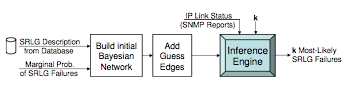
\includegraphics[width=0.5\textwidth]{Fig8}
\end{figure}

\begin{figure}[h!]
  \caption{Shrink's network model}
  \centering
    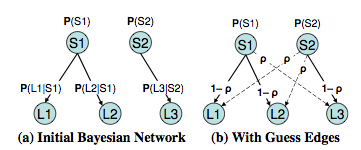
\includegraphics[width=0.5\textwidth]{Fig9}
\end{figure}

if $E_k$ denotes the event that at most k SRLGs failed within any hour, there are exactly k combinations of n possible SRLG assignmentsthat satisfy $E_k$. Given the observed link status, shrink algorithm greedily picks the most likely SRLG assignment in $E_k$; i.e., it picks $(S_1,.....,Sn)$ $\in$ $\{0,1\}^n$ such that: \\
$arg \underset{S_1,....,S_n}{max} P(S_1,.....,S_n|L_1,....L_n)$ subject to number of \{$S_i$=1\} $\leq$ k \\
There are fewer than $n^k$ value assignments in $E_k$, and for each assignment $P(S_1,...,S_n|L_1,...,L_m)$ can be computed in O(m + n) time, where m is the number of IP links and n is the number of SRLGs. So, Shrink’s running time is O($n^k$ ∗(m+n)). k=3 is a valid case for a wide range of ISP network sizes and SRLG failure probabilities and when k$\geq$3 the hypothesis performance is exponential. 

\subsection{Misc approaches}

There are several other approaches to fault localization like codebook approach which uses hamming distances to find the fault and also context free grammer which allows xpressions to be built from subexpressions, may be effectively used to represent a hierarchically organized communication system. However these are not discussed in this papaer due to the poor applicability to the real world systems and poor performance of these approaches. \cite{Calo:95}, \cite{Kliger:95}, \cite{Yemini:1996} are papers that discuss about these techiniques.

\section{Paper 1: Toward Optimal Network Fault Correction in Externally Managed Overlay Networks}
\cite{pclee:07} Paper 1 is an end-to-end approach of inferring probabilistic data-forwarding failures in an externally managed overlay network, where overlay nodes are independently operated by various administrative domains. The optimization goal is to minimize the expected cost of correcting (i.e., diagnosing and repairing) all faulty overlay nodes that cannot properly deliver data. Instead of first checking the most likely faulty nodes as in conventional fault localization problems it chooses a {\it candidate node} proceed based on a potential heuristic function and is bound to infer correctly atleast 95\% of the time.

\cite{Katzela:95}, \cite{Sethi:04} and \cite{Kandula:05} state of the art techniques that diagnose (i.e detect and localize) the components that are root causes of the network faults, however they do not focus on the {\it network fault correction} that is not only diagnosis but also considering the repair and checking costs. \cite{pclee:07} conveniently outperforms all of them and tries to derive a strategy for efficient network fault correction at minimum cost. 

Another set of research papers focus purely on the failure detection of network faults \cite{Zhuang:05}, \cite{Mizrak:05} and \cite{Avramopoulos:04} uses distributed techniques and all networks nodes to collaboratively achieve the fault detection. \cite{Avramopoulos:04} uses inspection on packets from previous hop and reports when founded corruption. The problem with this approach is that an inspection logic or monitoring points have to be setup across the network and incurs heavy costs and different administration domains prove to be obstacle in the above cases too. 

Paper1 considers and end-end inference approach using end-end measurements, infers components that are faulty in forwarding data. This applies perfectly to the scenario like CAN\cite{Ratnasamy:01} and CHORD\cite{Stoica:01} where each overlay node builds a routing tree with itself as a root and in this setting every root to leaf path is monitored to find faulty path and anamolous behaviours on the path. One anamoulous behaviour could be number of correct packets bot being delivered in a fixed time period, such a validation could prove to be very important in QOS factor.  The authors are particular interested in diagonize and repairing faulty nodes in overlay networks like RON\cite{Andersen:01}, SON\cite{Duan:03} and SOS\cite{Misra:04}. The proposed fault correction mechanism suits well to this type of  networks. 

\subsection{Problem Formulation}
\cite{pclee:07} considers a logical tree as T=$(N,\{{p_i}\},\{{c_i}\}),$ where N is the set of overlay nodes, $p_i$ is the failure probability of node i$\in$N, and $c_i$ is the checking cost of deciding if node i$\in$N is faulty. Overlay set node N provides a topology information and sequence of nodes. The construction of failure probabilities and cost probabilities depend on Failure model and Cost model.

{\bf Failure Model} focus on the nodes that cannot forward data or fails to comply with a QOS because of which packets get dropped or fails to get delivered. Focus mainly stands on fail-stop failues like power outages, full transmission queues, hardware errors and route misconfigurations. The failure probabilities are calculated using statistical measurements of reliability indexes of node elements(vulnerability modelling).  Authors also performed analysis of the  mechanism under inaacurate probabilities and is provide in the results section of this paper. Important consideration to be made is that failure probabilities of nodes are independent of each other. 

{\bf Cost Model} provides the checking costs using personnel hours, wages and time effort that goes into debugging the problem or even the cost of the equipment. Important cirteria to be noted in the cost model the repair costs are not conisdered as eventually every fault has to be repaired. $p_i$ and $c_i$ can be any values between [0,1] and [0,$\infty$].

Each node in a logical tree T is classified as fault or non-faulty. and definitions are being made on each root to leaf path that exhibits an anamalous behaviour. Since an end-to-end inference mechanism is being made we only know that something is wrong with the path rather than which node is at fault. Each node in T is referred to as {\it bad} if it is faulty and {\it good} if it is non-faulty and a path in T is bad if it has atleast one {\it bad} node. An important consideration is that the node behaviour remains the same across all the paths as only fail-stop considerations are being made. 

Given a logical tree T we can infer the good path and bad paths by end to end inference mechanism, for example root can send a probe and collect all measurement results. We now create a bad Tree by pruning of all the good paths form the logical tree and also call it T with abuse of notation. Bad tree now becoms input to the inference algorithm which determines which set of nodes to be corrected(checked and repaired).

The optimization goal of this paper is to minimize the expected cost of correcting all faulty nodes in a given tree. repairing cost is not considered as eventually all the nodes have to be repaired and any strategy that is employed will eventually correct all the nodes. Here we focus only on the sequential case as checking the nodes in parallel doesnt improve the total expected checking cost so the inference algorithm only return one single node that is supposed to be the best node to check first. The best node is the first node that is from a diagnostic sequence {\it S} = $\{l_1,l_2,....,l_N\}$ and gives us {\it N!} diagnositic sequences.

When a particular node {\it $l_i$} lies on a bad path we do no know whether it is a good node or a bad node but if it is on a good node we know for sure it is a good node. {\it $l_i$}  gets {\it checked or skipped} based on the examination of the node. Thus we can summarize the total cost of checking a tree {\it T} is given by  \\
$\underset{i=1}{\overset{|N|}{\sum}} c_{l_i} Pr(node\ l_i\ is\ checked\ | \ nodes\ l_1,...,l_{i-1}\ known\ to\ be\ good)$ \\
So the best node would be the first node in the diagnosis sequence and the inference works on the current topolgy to indetify this node and when the node is corrected the revised topology is fed into the inference algorithm to output the next node. The total complexity of calculating the expected cost of a diganosis sequence is O($n^3$) and since there are n! differenct sequences, the brute force approach has a complexity of O($n^3$n!). The complexity and the way to calculate the total cost for the diagnostic sequence is mentioned in Appendix A of \cite{pclee:07}. In the interest of space and lenth only the highights are being mentioned here.

{\bf Conditional Failure Probabilties}: the nodes in T by 1 to $|$N$|$ in breadth- first-search order. $T_i$ is the subtree rooted at node i. $C_i$ is the set such that k$\in$$C_i$ if node k is a   child node of {\it i}. thus conditional failure probability is given by bayesian probability rule where Pr($X_i$) is the independent failure probability of a node, and Pr($T_1$) is the probability of the tree is bad at root, $Pr(T_1|X_i)$ is the probability that a tree is a bad tree upon the event that a node is bad. \\
$Pr(X_i|T_1) = \frac{Pr(T_1|X_i)Pr(X_i)}{Pr(T_1)}$ by baye's rule.\\
where\\
$Pr(T_i) = p_i+(1-p_i) \underset{k{\in}C_i}{\pi}Pr(T_k) , \forall i \in [1,|N|]$\\
\\

\[
 Pr(T_i|X_j) =
  \begin{cases}
   Pr(T_i) & \text{if } i > j \\
   1       & \text{if } i=j \\
   p_i+(1-p_i)  \underset{k{\in}C_i}{\pi} Pr(T_k|X_j)  & \text{if } i<j
  \end{cases}
\] \\

The idea here is that a subtree $T_i$ is bad if either the node itself is bad or node {\it i} is good and the subtree rooted at {\it i} is bad. Using dyanmic programming the above equation can be computed in O($N^2$) which is the conditional failure probabitlity of a node. 

{\bf Expected Cost of  a Diagnosis Sequence}: Let ${T_{l_i}}^D$ be the event that the subtree rooted at node ${l_i}$ is a bad tree after nodes ${{l_1},...,{l_{i-1}}}$ have been examined (i.e., checked or skipped). Let ${A_{l_i}}^D$ be the event that every ancestor j of node ${l_i}$, such that j $\in\{l_{i+1},...,l_{|N|}\}$ (i.e., node j is examined after node ${l_i}$), is a good node. Since every node is examined in a sequential way in the diagnosis sequence, when $l_i$ is examined, nodes $l_1,....,l_{i-1}$ have been examined and they are good. Thus, \\
$Pr({T_{l_i}}^D) = Pr(T_{l_i}|p_{l_1}= ... = p_{l_{i-1}} = 0)$, and \\
$Pr({A_{l_i}}^D) = Pr(A_{l_i}|p_{l_1}= ... = p_{l_{i-1}} = 0)$ \\
Where $T_{l_i}$ is the event that the subtree rooted at node $l_i$ is bad, and $A_{l_i}$ is the event that all ancestors of node $l_i$ are good. If the subtree rooted at node $l_i$ remains a bad tree or at least one of the ancestors of node $l_i$ is a bad node, then node $l_i$ still lies on bad path and needs to be checked. Thus, \\
$ Pr(node\ l_i\ is\ checked| T, nodes\ l_1,...,l_{i-1} known\ to\ be\ good)$ \\
$=Pr({T_{l_i}}^D \cup \neg{{A_{l_i}}^D} | T)$\\
Thus the expected cost of S given that T is a bad tree is: \\
\center$ \underset{i=1}{\overset{n}{\sum}} c_{l_i} Pr({T_{l_i}}^D \cup \neg{{A_{l_i}}^D} | T)$\\
Brute force algorithm which inspects all the sequences is given in figure 10. This algorithm makes a good reference for comapring against the heuristic based ones.

\begin{figure}[h!]
  \caption{Bruce Force Algorithm}
  \centering
    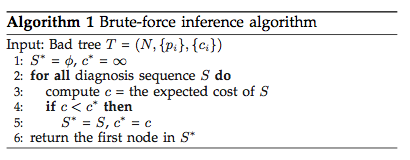
\includegraphics[width=0.5\textwidth]{Fig10}
\end{figure}

\subsection{Naive Heuristics for Inference Algorithm}
Intuitively the best node returned by the inference algorithm can be either based on the highest conditional failure probabiltiy or checking cost.  The authors provided a simple counter example in which neither the selection of node based on conditional failure probability nor the one selected based on checking cost gave the optimal solution. The three heuristics authors chose naively are (1) {\it Naive_Prob} (2) {\it Naive_Cost} (3) {\it Naive_Prob_Cost} . Based on the experimental setup where a 200 bad trees are tested with the three heuristic mentioned above with varying probabiltiy and cost distributions. Depending on the distributions of $p_i$ and $c_i$, the proportion of instances where the best choice is made can be as low as 10\% for Naive-Prob and Naive-Cost  and less than 55\% for Naive-Prob-Cost.
\begin{figure}[h!]
  \caption{Naive-Prob, Naive-Cost, and Naive-Prob-Cost performance}
  \centering
    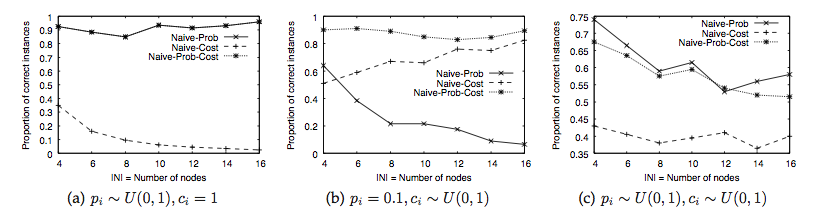
\includegraphics[width=0.5\textwidth]{Fig11}
\end{figure}

\subsection{Candidate Node}
The authors show that instead of selecting a node to test based on naive choices we should select a {\it candidate node} based on the maximization of a {\it potential function}. Let $A_i$ be the event that the ancestors of node {\it i} are all good. If node {\it r} is the root node, then we let $A_r$ be always true and $Pr(A_r) = 1$. The potential of a candidate node is calculated using the formula. \\
                        \center $\phi({\it i,T)} = \frac{Pr(T|X_i,A_i)p_i}{c_i(1-p_i)}$
\appendix
%\bibliographystyle{abbrv}
%\bibliography{sigproc}

\input{sensys10-sample-10pt.bbl}

\end{document}


\end{document}


\end{document}


\end{document}
